
%% abtex2-modelo-trabalho-academico.tex, v-1.9.7 laurocesar
%% Copyright 2012-2018 by abnTeX2 group at http://www.abntex.net.br/ 
%%
%% This work may be distributed and/or modified under the
%% conditions of the LaTeX Project Public License, either version 1.3
%% of this license or (at your option) any later version.
%% The latest version of this license is in
%%   http://www.latex-project.org/lppl.txt
%% and version 1.3 or later is part of all distributions of LaTeX
%% version 2005/12/01 or later.
%%
%% This work has the LPPL maintenance status `maintained'.
%% 
%% The Current Maintainer of this work is the abnTeX2 team, led
%% by Lauro César Araujo. Further information are available on 
%% http://www.abntex.net.br/
%%
%% This work consists of the files abntex2-modelo-trabalho-academico.tex,
%% abntex2-modelo-include-comandos and abntex2-modelo-references.bib
%%

% ------------------------------------------------------------------------
% ------------------------------------------------------------------------
% abnTeX2: Modelo de Trabalho Academico (tese de doutorado, dissertacao de
% mestrado e trabalhos monograficos em geral) em conformidade com 
% ABNT NBR 14724:2011: Informacao e documentacao - Trabalhos academicos -
% Apresentacao
% ------------------------------------------------------------------------
% ------------------------------------------------------------------------

\documentclass[
	% -- opções da classe memoir --
	12pt,				% tamanho da fonte
	openright,			% capítulos começam em pág ímpar (insere página vazia caso preciso)
	oneside,			% para impressão em recto e verso. Oposto a oneside
	a4paper,			% tamanho do papel. 
	% -- opções da classe abntex2 --
	%chapter=TITLE,		% títulos de capítulos convertidos em letras maiúsculas
	%section=TITLE,		% títulos de seções convertidos em letras maiúsculas
	%subsection=TITLE,	% títulos de subseções convertidos em letras maiúsculas
	%subsubsection=TITLE,% títulos de subsubseções convertidos em letras maiúsculas
	% -- opções do pacote babel --
	english,			% idioma adicional para hifenização
	brazil				% o último idioma é o principal do documento
	]{abntex2}

% ---
% Pacotes básicos 
% ---
\usepackage{float}
\usepackage{lmodern}			% Usa a fonte Latin Modern			
\usepackage[T1]{fontenc}		% Selecao de codigos de fonte.
\usepackage[utf8]{inputenc}		% Codificacao do documento (conversão automática dos acentos)
\usepackage{indentfirst}		% Indenta o primeiro parágrafo de cada seção.
\usepackage{color}				% Controle das cores
\usepackage{graphicx}			% Inclusão de gráficos
\usepackage{microtype} 			% para melhorias de justificação
\usepackage{verbatim}           % para comentários em massa
\usepackage{multirow}
\usepackage{epsfig}
\usepackage{caption}
\usepackage{makecell}
\usepackage{svg}
\usepackage{amsmath}
\usepackage{tikz}
\def\checkmark{\tikz\fill[scale=0.4](0,.35) -- (.25,0) -- (1,.7) -- (.25,.15) -- cycle;} 
\usepackage{makecell}
\usepackage{tabulary}
\usepackage{pdfpages}
\usepackage{fancyhdr}
\usepackage{xcolor,colortbl}
\usepackage{subfig}
% ---
		
% ---
% Pacotes adicionais, usados apenas no âmbito do Modelo Canônico do abnteX2
% ---
\usepackage{lipsum}				% para geração de dummy text
% ---

% ---
% Pacotes de citações
% ---
\usepackage[brazilian,hyperpageref]{backref}	 % Paginas com as citações na bibl
\usepackage[alf]{abntex2cite}	% Citações padrão ABNT
\citebrackets()

% --- 
% CONFIGURAÇÕES DE PACOTES
% --- 

% ---
% Configurações do pacote backref
% Usado sem a opção hyperpageref de backref
\renewcommand{\backrefpagesname}{Citado na(s) página(s):~}
% Texto padrão antes do número das páginas
\renewcommand{\backref}{}
% Define os textos da citação
\renewcommand*{\backrefalt}[4]{
	\ifcase #1 %
		Nenhuma citação no texto.%
	\or
		Citado na página #2.%
	\else
		Citado #1 vezes nas páginas #2.%
	\fi}%
% ---

% ---
% Informações de dados para CAPA e FOLHA DE ROSTO
% ---
\titulo{Generative Adversarial Networks para a identificação de genes \textit{housekeeping} mediante classificação em RNA-seq}
\autor{Edwin Jahir Rueda Rojas}
\local{Belém}
\data{2019}
\orientador{Prof. Dr. Jefferson Magalhães de Morais}
\coorientador{Prof. Dr. Rommel Ramos}
\instituicao{Universidade Federal do Pará}
\instituicaounidade{Instituto de Ciências Exatas e Naturais}
\instituicaosubunidade{Programa de Pós-Graduação em Ciência da Computação}


\tipotrabalho{Tese (Doutorado)}
% O preambulo deve conter o tipo do trabalho, o objetivo, 
% o nome da instituição e a área de concentração 
\preambulo{Qualificação de Mestrado apresentada ao Programa de Pós-Graduação em Ciência da Computação do Instituto de Ciências Exatas e Naturais como requisito parcial para obtenção do título de Mestre em Ciência da Computação.}
% ---


% ---
% Configurações de aparência do PDF final

% alterando o aspecto da cor azul
\definecolor{blue}{RGB}{41,5,195}

% informações do PDF
\makeatletter
\hypersetup{
     	%pagebackref=true,
		pdftitle={\@title}, 
		pdfauthor={\@author},
    	pdfsubject={\imprimirpreambulo},
	    pdfcreator={LaTeX with abnTeX2},
		pdfkeywords={abnt}{latex}{abntex}{abntex2}{trabalho acadêmico}, 
		colorlinks=true,       		% false: boxed links; true: colored links
    	linkcolor=black,          	% color of internal links
    	citecolor=black,        		% color of links to bibliography
    	filecolor=black,      		% color of file links
		urlcolor=black,
		bookmarksdepth=4
}
\makeatother
% --- 

% ---
% Posiciona figuras e tabelas no topo da página quando adicionadas sozinhas
% em um página em branco. Ver https://github.com/abntex/abntex2/issues/170
\makeatletter
\setlength{\@fptop}{5pt} % Set distance from top of page to first float
\makeatother
% ---

% ---
% Possibilita criação de Quadros e Lista de quadros.
% Ver https://github.com/abntex/abntex2/issues/176
%
\newcommand{\quadroname}{Quadro}
\newcommand{\listofquadrosname}{Lista de quadros}

\newlistof{listofquadros}{loq}{\listofquadrosname}
\newlistentry{quadro}{loq}{0}

% configurações para atender às regras da ABNT
\setfloatadjustment{quadro}{\centering}
\counterwithout{quadro}{chapter}
\renewcommand{\cftquadroname}{\quadroname\space} 
\renewcommand*{\cftquadroaftersnum}{.\hfill}

\setfloatlocations{quadro}{hbtp} % Ver https://github.com/abntex/abntex2/issues/176
% ---

% --- 
% Espaçamentos entre linhas e parágrafos 
% --- 

% O tamanho do parágrafo é dado por:
\setlength{\parindent}{1.3cm}

% Controle do espaçamento entre um parágrafo e outro:
\setlength{\parskip}{0.2cm}  % tente também \onelineskip

% ---
% compila o indice
% ---
\makeindex
% ---

% ----
% Início do documento
% ----
\begin{document}

% Seleciona o idioma do documento (conforme pacotes do babel)
%\selectlanguage{english}
\selectlanguage{brazil}

% Retira espaço extra obsoleto entre as frases.
\frenchspacing 

% ----------------------------------------------------------
% ELEMENTOS PRÉ-TEXTUAIS
% ----------------------------------------------------------
% \pretextual

% ---
% Capa
% ---
\imprimircapa
% ---

% ---
% Folha de rosto
% (o * indica que haverá a ficha bibliográfica)
% ---
\imprimirfolhaderosto*
% ---

% ---
% Inserir a ficha bibliografica
% ---

% Isto é um exemplo de Ficha Catalográfica, ou ``Dados internacionais de
% catalogação-na-publicação''. Você pode utilizar este modelo como referência. 
% Porém, provavelmente a biblioteca da sua universidade lhe fornecerá um PDF
% com a ficha catalográfica definitiva após a defesa do trabalho. Quando estiver
% com o documento, salve-o como PDF no diretório do seu projeto e substitua todo
% o conteúdo de implementação deste arquivo pelo comando abaixo:
%
% \begin{fichacatalografica}
%     \includepdf{fig_ficha_catalografica.pdf}
% \end{fichacatalografica}

\begin{comment}

\begin{fichacatalografica}
	\sffamily
	\vspace*{\fill}					% Posição vertical
	\begin{center}					% Minipage Centralizado
	\fbox{\begin{minipage}[c][8cm]{13.5cm}		% Largura
	\small
	Solicite sua ficha catalográfica em: \url{http://bcficat.ufpa.br/}
	\end{minipage}}
	\end{center}
\end{fichacatalografica}

\end{comment}

% ---

% ---
% Inserir errata
% ---
%\begin{errata}
%Elemento opcional da %\cite{NBR14724:2011}. Exemplo:

%\vspace{\onelineskip}

%FERRIGNO, C. R. A. \textbf{Tratamento de neoplasias ósseas apendiculares com
%reimplantação de enxerto ósseo autólogo autoclavado associado ao plasma
%rico em plaquetas}: estudo crítico na cirurgia de preservação de membro em
%cães. 2011. 128 f. Tese (Livre-Docência) - Faculdade de Medicina Veterinária e
%Zootecnia, Universidade de São Paulo, São Paulo, 2011.

%\begin{table}[htb]
%\center
%\footnotesize
%\begin{tabular}{|p{1.4cm}|p{1cm}|p{3cm}|p{3cm}|}
%  \hline
%   \textbf{Folha} & \textbf{Linha}  & \textbf{Onde se lê}  & \textbf{Leia-se}  \\
%    \hline
%    1 & 10 & auto-conclavo & autoconclavo\\
%   \hline
%\end{tabular}
%\end{table}

%\end{errata}
% ---

% ---
% Inserir folha de aprovação
% ---

% Isto é um exemplo de Folha de aprovação, elemento obrigatório da NBR
% 14724/2011 (seção 4.2.1.3). Você pode utilizar este modelo até a aprovação
% do trabalho. Após isso, substitua todo o conteúdo deste arquivo por uma
% imagem da página assinada pela banca com o comando abaixo:
%
% \begin{folhadeaprovacao}
% \includepdf{folhadeaprovacao_final.pdf}
% \end{folhadeaprovacao}
%
\begin{folhadeaprovacao}

  \begin{center}
    {\ABNTEXchapterfont\large\imprimirautor}

    \vspace*{\fill}\vspace*{\fill}
    \begin{center}
      \ABNTEXchapterfont\bfseries\Large\imprimirtitulo
    \end{center}
    \vspace*{\fill}
    
    \hspace{.45\textwidth}
    \begin{minipage}{.5\textwidth}
        \imprimirpreambulo
    \end{minipage}%
    \vspace*{\fill}
   \end{center}
        
   Conceito: \rule{3cm}{.1pt}
   
   \imprimirlocal, <dia> de <mes> de 2019.
   
   \vspace{1cm}
   \begin{center}
   BANCA EXAMINADORA
   \end{center}
    

   \assinatura{\textbf{\imprimirorientador} - Orientador \\ UFPA}
   \assinatura{\textbf{\imprimircoorientador} - Coorientador \\ UFPA}
   \assinatura{\textbf{Prof.} \\ UFPA}
   \assinatura{\textbf{Prof.} \\ UFPA}
   %\assinatura{\textbf{Nome Convidado 3} \\ SIGLA INSTITUIÇÃO}
      

  
\end{folhadeaprovacao}
% ---

% ---
% Dedicatória
% ---
%\begin{dedicatoria}
%   \vspace*{\fill}
%   \centering
%   \noindent
%   \textit{ Dedico este trabalho a pessoa que há 11 anos vem sendo minha maior fonte de motivação para enfrentar e superar todos os desafios que a vida vem colonado em meu caminho. \\Com amor para meu filho Arthur Santos.} \vspace*{\fill}
%\end{dedicatoria}
% ---

% ---
% Agradecimentos
% ---
%\begin{agradecimentos}

%...

%\end{agradecimentos}
% ---

% ---
% Epígrafe

% ---
%\begin{epigrafe}
%   \vspace*{\fill}
%	\begin{flushright}
%		\textit{“Quando a neve branca cai e os ventos frios do inverno sopram, o lobo sozinho morre, mas a alcateia sobrevive.”\\
%		Eddard Stark - Game of Thrones}
%	\end{flushright}
%\end{epigrafe}
% ---

% ---
% RESUMOS
% ---
% resumo em português
\setlength{\absparsep}{18pt} % ajusta o espaçamento dos parágrafos do resumo
\begin{resumo}
Os \textit{genes housekeeping} (HKG) ou genes de referência na biologia molecular, são genes constituintes necessários para a manutenção da função celular básica e eles estão expressos em todas as células de um organismo, por tanto, sua expressão é vital para a sobrervivência

 \textbf{Palavras-chave}: Generative Adversarial Networks, Deep Learning, genes, RNA-seq.
\end{resumo}

% resumo em inglês
\begin{resumo}[Abstract]
 \begin{otherlanguage*}{english}
   Resume

   \vspace{\onelineskip}
 
   \noindent 
   \textbf{Keywords}: Information visualization, charts textual description templates, vocalization.
 \end{otherlanguage*}
\end{resumo}

% ---

% ---
% inserir lista de ilustrações
% ---
\pdfbookmark[0]{\listfigurename}{lof}
\listoffigures*
\cleardoublepage
% ---

% ---
% inserir lista de quadros
% ---
%\pdfbookmark[0]{\listofquadrosname}{loq}
%\listofquadros*
%\cleardoublepage
% ---

% ---
% inserir lista de tabelas
% ---
\pdfbookmark[0]{\listtablename}{lot}
\listoftables*
\cleardoublepage
% ---

% ---
% inserir lista de abreviaturas e siglas
% ---
%\begin{comment}

\begin{siglas}
  \item[GAN] \textit{Generative Adversarial Networks} (Redes Geradoras Adversárias)
  \item[HKG] \textit{Housekeeping}
  \item[RNA-seq] Sequenciamento de RNA
  \item[AI] \textit{Artificial Intelligence} (Inteligência Artificial)
\end{siglas}

%\end{comment}
% ---

% ---
% inserir lista de símbolos
% ---
%\begin{simbolos}
 %\item[$ \Gamma $] Letra grega Gama
 %\item[$ \Lambda $] Lambda
  %\item[$ \zeta $] Letra grega minúscula zeta
  %\item[$ \in $] Pertence
%\end{simbolos}
% ---

% ---
% inserir o sumario
% ---
\pdfbookmark[0]{\contentsname}{toc}
\tableofcontents*
\cleardoublepage
% ---
% ----------------------------------------------------------
% ELEMENTOS TEXTUAIS
% ----------------------------------------------------------
\textual

% ----------------------------------------------------------
% Introdução (exemplo de capítulo sem numeração, mas presente no Sumário)
% ----------------------------------------------------------
\chapter{Introdução}
% ----------------------------------------------------------
A Biologia computacional ou Bioinformática, é a interdiciplina entre a Biologia e a Informática, a qual tem uma abordagem derivado da Ciência da Computação e da Estatística, entre outras disciplinas para o entendimento de diversos problemas com dados em larga escala ~\cite{MLuscombe}. Assim, a Computação consegue resolver os problemas presentes na Biologia, como por exemplo o problema da identificação dos genes \textit{HKG}, o qual será tratado nesta pesquisa.

Os genes \textit{HKG} são genes constituintes necessários para a manutenção da função celular básica e eles estão expressos em todas as células de um organismo. Por tanto, sua expressão é vital para a sobrervivência. Assim, estes genes são empregados em controles internos em pesquisas de análises de expressão gênica~\cite{valente2009selection}. 

Devido a sua importância, os genes \textit{HKG} são atualmente os geradores de um grande número de pesquisas, e é que para os pesquisadores é importante a identificação deles. Na expressão gênica uma técnica que permite seu estudo dentro de um organismo é o \textit{quantitative real-time} PCR (qRT-PCR), o qual fornece uma quantificação precisa e reproduzível de cópias genéticas ~\cite{heid1996real}. Neste abordagem, os genes \textit{HKG} são empregrados para a normalização dos resultados do qRT-PCR ~\cite{de2008identification}.

Por sua grande aplicação, a identificação de genes \textit{HGK} é essencial, para isso, atualmente são empregados métodos os quais avaliam a estabilidade destes genes em diferentes condições de estresse, tendo em conta, que para que seja considerado o gene como \textit{HKG}, este tem que ser avalidado em dois o mais testes ~\cite{rocha2015bacterial}, o que implica um custo alto de recursos econômicos e tempo de laboratório.

Na atualidade, métodos de AI tem sido feitos para a identificação de genes \textit{HKG in-silico}. Diferentes abordagens foram empregadas na literatura para essa identificação, uma delas é a \textit{Ratio Statistics Based Normalization Strategy}, a qual emprega modelos gaussianos para conseguir ter uma probabilidade para dizer se um gene pode ser candidato a \textit{HKG}, para isso o modelo é treinado com genes que na literatura são conhecidos como não \textit{HKG}, tratando assim, os genes \textit{HKG} como anomalias ~\cite{sengupta2015computational}.

Outra abordagem para a identificação dos genes \textit{HGK} é o qual emprega algoritmos de agrupamento (\textit{Clustering}), estes algoritmos conseguem agrupar diferentes tipos de genes dependendo de certas métricas de validação, sendo a métrica de distância a mais empregada, encontrando assim, grupos de genes que podem ser candidatos a \textit{HKG}, devido a que tão pertos estão eles dos genes considerados \textit{HKG}  ~\cite{berghoff2017rna}.

Ao falar de AI, falamos sobre a construção de algoritmos os quais melhoram com a experiência. Se diz que um algoritmo aprende de uma experiência E com respeito a uma classe de tarefas T e com medida de desempenho P, se seu desempenho em tarefas T, medido por P, melhora com a experiência E ~\cite{jordan2015machine}.

Na abordagem de algoritmos de AI surge o problema de ter a suficiente quantidade de dados para ter um desempenho razoavél, mas isso não basta, além disso, a quantidade de dados tem que estar equilibrado, já que não é suficiente ter uma quantidade grande de dados se esses quantidades não forem proporcionais ~\cite{visa2005issues}. Este é o problema da identificação dos genes \textit{HGK} quando o abordagem é mediante a classificação destes, embora há muitos genes, só uma pouca parte deles estão avalidados na literatura como \textit{HKG}, é por isso, que ao desenvolver um algoritmo de AI para resolver este problema mediante a classificação, o algoritmo não vai ter um bom desempenho já que os dados da classe \textit{HKG} serão menores que os dados da classe não \textit{HKG}.

Embora estes dados podem ser tradados assim mediante ajustes nos algoritmos de AI, recentemente, novos algoritmos foram desenvolvidos para aumentar as classes de dados que apresentam uma pequena quantidade em relação aos demais. Na área das redes neurais, surgiu uma técnica chamada \textit{Generative Adversarial Networks} (GAN's), a qual mediante um processo adversário é capaz de treinar duas redes, uma chamada rede geradora e outra chamada rede discriminadora, o objetivo é que a rede geradora consegue gerar dados semelhantes aos pertencentes à classe minoritária, aumentando assim sua quantidade e tendo como efeito principal o aumento do rendimento dos algoritmos de AI, mais especialmente com os algoritmos de classificação ~\cite{goodfellow2014generative}.

Feito o aumento da classe minoritária, os dados balanceados já podem ser tratados mediante uma técnica de AI de aprendizado supervisionado, o qual treina um algoritmo com dados os quais já estão categorizados. Para melhorar o desempenho, o algoritmo tenta minimizar o erro mediante a minimização de uma função de custo. Assim, dado um novo dado de entrada, o algoritmo vai dizer a que categoria ou classe ele pertence.

Neste trabalho é apresentada uma abordagem para a identificação de genes \textit{HKG in-silico} mediante a abordagem de AI com algoritmos de classificação em aprendizado supervisionado, para isso, é resolvido o problema de desequilíbrio das classes mediante a geração de mais dados através da implementação das redes GAN's.
%-----Exemplo de citação-----
%cita ~\cite{Savva2011}.


\section{Justificativa}

Na actualidade existem métodos de AI os quais conseguem selecionar candidatos a genes \textit{HKG in-silico}, tendo assim algoritmos de agrupamento (\textit{clustering}) e algoritmos baseados em seleção de anomalias. O objetivo de usar essas propostas é para atenuar o teste \textit{in-vitro} dos genes, o qual precisa de tempo em laboratorio e de recursos económicos. Mas, o rendimento destes algoritmos é baseado nos dados de treinamento utilizados, ou seja, é basado na diversidade e quantidade dos dados utlizados na hora de treinar os modelos. Por exemplo, para os algoritmos de agrupamento, estes foram treinados com poucos genes \textit{HKG}, assim mesmo, para os algoritmos de seleção de anomalias, tendo este último a ventagem de ser feito para quando os dados de uma classe são poucos respeito a outra classe, mais, ainda assim, o modelo treinado vai mudar seus parâmetros baseado só em um pequeno conjunto de dados o qual pode que não represente a diversidade dos dados.

Devido a que o conjunto de dados do treinamento dos algoritmos é pequeno na classe dos genes \textit{HKG} em relação à classe dos genes não \textit{HKG}, isso influencia no desempenho dos algoritmos de AI, já que um algoritmo treinado com poucos dados de uma certa classe, é um algoritmo cujo resultado não será o mais generalizado possivel e é um algoritmo o qual sua resposta pode estar viciada só por a classe com a maior quantidade de dados.

A motivação deste trabalho é tentar atenuar o problema do desequilíbrio dos dados, para assim, ter uma identificação de genes \textit{HKG} mediante AI mais robusta. Para isso, vai ser tratado o problema do desequilíbrio da classe \textit{HKG} mediante técnicas de geração de dados, é aí, onde as redes GANs vão ser empregadas, elas vão conseguir imitar a distribuição dos dados da classe minoritária para assim aumentar sua relação com respeito aos dados não \textit{HKG}, para depois ser feito um classificador o qual vai dizer se um novo gene pode ser ou não cadidato a \textit{HKG}.

\section{Objetivos}

\subsection{Objetivo Geral}
Identificação de possíveis novos genes \textit{housekeeping in-silico} mediante algoritmos de Aprendizado de Máquina com dados de expressão gênica.

\subsection{Objetivos Específicos}
\begin{itemize}
    \item Realizar uma revisão bibliográfica sobre modelos de identificação de genes \textit{in-silico}.
    \item Escolher os genes \textit{housekeeping} que serão empregados para seu estudo.
    \item Criar uma arquitetura de rede GAN para a geração de novos genes \textit{housekeeping} e avaliar seu desempenho.
    \item Criar um algoritmo de classificação de genes mediante AI e avaliar seu desempenho.
\end{itemize}

\section{Organização do Texto}

\chapter{TRABALHOS RELACIONADOS}
A tarefa da seleção de genes candidatos a \textit{HKG in-silico} empregando AI é uma tarefa a qual está tendo uma abordagem importante devido ao impacto que este tem na redução do custo econômico e do tempo empregado no laboratório. Tem surgido iniciativas empregando métodos de agrupamento, por exemplo, no trabalho de ~\cite{xia2017identification} é feita uma seleção de genes \textit{HKG} baseado no \textit{software Primer Premier} o qual emprega o algoritmo dos vizinhos mais próximos para dar uma estimativa dos genes que podem ser candidatos a \textit{HKG}

\chapter{Fundamentação Teórica}

Nesta seção são apresentados os conceitos fundamentais relacionados ao desenvolvimento deste estudo, assim como, estudos já desenvolvidos na área.

\section{Genes \textit{Housekeeping}}

\subsection{Identificação de genes}
\section{Aprendizado de Máquina}
Na área da AI, o Aprendizado de Máquina se refere ao fato de construir algoritmos os quais melhoram com a experiência, ou seja, se diz que um computador aprende de uma experiência \textbf{E} com respeito à umas tarefas \textbf{T} com medida de desempenho \textbf{P}, se seu desempenho nas tarefas \textbf{T}, medido por \textbf{P}, melhora com a experiência \textbf{E} ~\cite{jordan2015machine}. Além disso, o Aprendizado de Máquina tem dois ramos importantes, o aprendizado supervisionado o qual vai ser empregado nesta pesquisa e estes são algoritmos feitos para quando os dados estão marcados, ou seja, são distinguíveis. E o aprendizado não supervisionado, que é quando os dados não são distinguíveis.

\subsection{Classificação com Aprendizado Supervisionado}
Na área de Aprendizado Supervisionado, a classificação é tratada quando se tem dados que estão rótulados e precisa-se criar um algoritmo que distinga estes rótulos. Para resolver este problema, é feito um problema de optimização matemática, o qual é um modelo que tem um conjunto de parâmetros: $$\theta = \theta_{0} + \theta_{1} + \dots + \theta_{n}$$
Os quais interagem com o conjunto de dados de entrada X e é dado um valor chamado de hipótese o qual prevê a probabilidade de que o dado pertence a uma classe: $$h_{\theta}(x) = classe, probabilidade$$
Como o objetivo é melhorar o algoritmo, é feita uma função de custo $J(\theta)$ na qual o parâmetro $\theta$ vai ser minimizado: $$\min_{\theta_{0}\dots \theta_{n}} J(\theta)$$

O proceso empregado para a criação do modelo de classificação é ilustrado na Figura~\ref{fig:classificacao}.

\begin{figure}[!h]
    \centering
    \caption{Modelo do proceso de criação do classificador.}
    %\includesvg[scale=.8]{figures/classificacao.svg}
    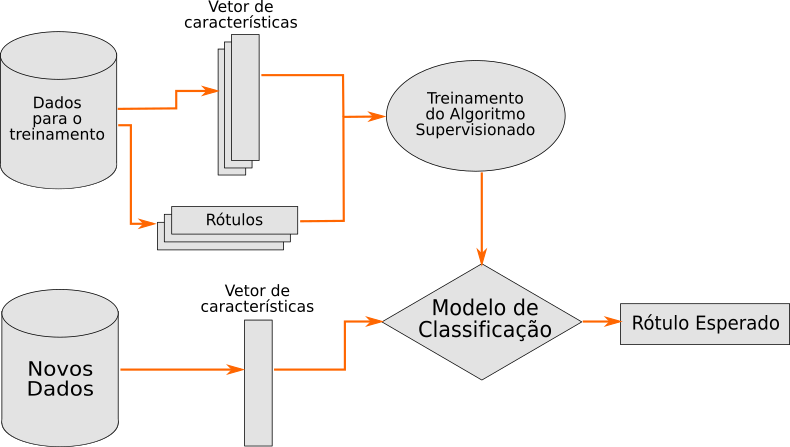
\includegraphics[scale=.7]{figures/classificacao.png}
    \caption*{Fonte: Autor}
    \label{fig:classificacao}
\end{figure}

\subsubsection{Métricas de avaliação}

\subsection{Redes Neurais Artificiais}

\subsubsection{Generative Adversarial Networks}

\subsubsubsection{Métricas de avaliação}



Nota-se a partir da literatura consultada que existem muitos trabalhos voltados a pessoas com deficiência visual que realizam a leitura dos modelos contendo os dados do gráfico, utilizando voz sintética, que geram o modelo textual, visando o público geral, ou até mesmo sugerem que exista uma ferramenta interativa e personalizável. Este trabalho propõe modelos de descrição textual para gráficos de barras e a avaliação dos modelos foi realizada não somente usando a vocalização da descrição textual com voz sintética, como também a interação por voz do usuário com o protótipo de uma aplicação.

\chapter{Metodologia}

As etapas deste trabalho estão especificadas conforme a Figura~\ref{fig:metodologia}.

\begin{figure}[!h]
\caption{Etapas da metodologia.}
%\centerline{\includegraphics[scale=.24]{figures/metod.png}}
\caption*{Fonte: Autor}
\label{fig:metodologia}
\end{figure}

\section{Normalização dos genes}

\section{Geração de novos genes mediante as GANs}



\begin{table}[hbtp]

\footnotesize
\centering
\settowidth\tymin{\textbf{Modelo}}
%\setlength\extrarowheight{2pt}
\caption{Modelos para vocalização de dados de gráficos de barras.}
\label{tab:modelos}

\begin{tabulary}{1\textwidth}{|C|J|}
\hline

    \textbf{Modelo} & 
    \textbf{Descrição Textual} \\
\hline
     \vspace{0.5cm}{1} & {Este é um gráfico de barras verticais. Seu título é \{título\}. A legenda do eixo y é denominada \{rótulo do eixo y\}. A legenda do eixo x é denominada \{rótulo do eixo x\}. A primeira barra é denominada \{nome da primeira barra\} e apresenta valor \{valor da primeira barra\}. ($\ldots$) A n-ésima barra é denominada \{nome da n-ésima barra\} e apresenta valor \{valor da n-ésima barra\}}   \\ \hline 
      \vspace{1.6cm}{2} & {Este é um gráfico de barras verticais agrupadas. Seu título é \{título\}. A legenda do eixo y é denominada \{rótulo do eixo y\}. A legenda do eixo x é denominada \{rótulo do eixo x\}. O gráfico é composto pelos grupos de barras \{nome do primeiro grupo de barras ($\ldots$) nome do n-ésimo grupo de barras\}. Cada grupo contém \{número de barras\} barras denominadas: \{nome da primeira barra, ($\ldots$), nome da n-ésima barra\}, que serão apresentadas nessa ordem. O primeiro conjunto de barras é denominado \{nome do primeiro grupo de barras\} e possui valores \{valor da primeira barra, ($\ldots$), valor da n-ésima barra\}. O segundo conjunto de barras é denominado \{nome do segundo grupo de barras\} e possui valores \{valor da primeira barra, ($\ldots$), valor da n-ésima barra\}.($\ldots$). O \{n-ésimo\} conjunto de barras é denominado \{nome do n-ésimo conjunto de barras\} e possui valores \{valor da primeira barra, ($\ldots$), valor da n-ésima barra\}}  \\ \hline
     \vspace{1.55cm}{3} &{Este é um gráfico de barras verticais agrupadas. Seu título é \{título\}. A legenda do eixo y é denominada \{rótulo do eixo y\}. A legenda do eixo x é denominada \{rótulo do eixo x\}. O gráfico é composto pelos grupos de barras: \{nome do primeiro grupo de barras, ($\ldots$), nome do n-ésimo grupo de barras\}. Cada grupo contém \{número de barras\} barras denominadas: \{nome da primeira barra, ($\ldots$), nome da n-ésima barra\}, nesta ordem. A série \{nome da primeira barra do primeiro grupo\} tem valores \{valorda primeira barra do primeiro grupo\} no grupo \{nome do primeiro grupo\}, ($\ldots$) e \{valor da primeira barra do n-ésimo grupo\} no grupo \{nome do n-ésimo grupo\}. ($\ldots$). A série \{nome da n-ésima barra do primeiro grupo\} tem valores \{valor da n-ésima barra do primeiro grupo\} no grupo \{nome do primeiro grupo\}, ($\ldots$) e \{valor da n-ésima barra do n-ésimo grupo\} no grupo \{nome do n-ésimo grupo\}.}\\ \hline
     \vspace{1.55cm}{4} & {Este é um gráfico de barras verticais. Seu título é \{título\}. A legenda do eixo y é denominada \{rótulo do eixo y\}. A legenda do eixo x é denominada \{rótulo do eixo x\}. A primeira barra é denominada \{nome da primeira barra\} e apresenta valor \{valor da primeira barra\}. ($\ldots$). A enésima barra é denominada \{nome da n-ésima barra\} e apresenta valor \{valor da n-ésima barra\}. ($\ldots$) Este é um gráfico de barras verticais. Seu título é \{título\}. A legenda do eixo y é denominada \{rótulo do eixo y\}. A legenda do eixo x é denominada \{rótulo do eixo x\}. A primeira barra é denominada \{nome da primeira barra\} e apresenta valor \{valor da primeira barra\}. ($\ldots$). A enésima barra é denominada \{nome da n-ésima barra\} e apresenta valor \{valor da n-ésima barra\}.}\\
   
    \hline
\end{tabulary}

\end{table}



\subsection{Avaliação da GAN}

\section{Classificação dos genes}

\subsection{Avaliação do classificador}

\chapter{Resultados Parciais}

Os resultados foram divididos de acordo com o tipo de avaliação: quantitativa e qualitativa. A análise quantitativa apresenta a quantidade de acertos e erros das perguntas respondidas pelos participantes, assim como a relevância estatística entre os testes 1 e 2 e as diferenças entre os modelos no teste 3. Também foram verificadas estatisticamente as diferenças entre os testes com e sem a possibilidade de interação. A análise qualitativa foi realizada a partir das opiniões dos voluntários sobre os testes realizados, onde emergiram categorias de significados que destacam pontos importantes sobre as características dos modelos.

\section{Análise Quantitativa}

O gráfico mosaico (\textit{mosaic chart}) da Figura~\ref{fig:mosaic} apresenta uma visão geral da acurácia obtida pelos participantes ao responder as questões referentes aos gráficos de cada teste. A acurácia foi dividida em três categorias: 0.0 (em vermelho) quando o participante erra completamente a questão; 0.5 (em amarelo) quando o participante acerta parcialmente a questão (por exemplo, responde apenas a metade do título do gráfico); e 1.0 (em verde) quando o participante acerta a questão por completo.

\begin{figure}[!h]
\caption{Taxa de acerto obtida pelos participantes para questões sobre os gráficos.}
%\centerline{\includegraphics[scale=.4]{figures/mosaicplot2.png}}
\caption*{Fonte: Autor}
\label{fig:mosaic}
\end{figure}

Analisando a Figura~\ref{fig:mosaic} percebe-se que os participantes erraram mais durante a realização do teste 2, principalmente as questões Q5 e Q6 relacionadas ao contexto do gráfico. Isto pode ter ocorrido porque no teste 2 os participantes tiveram um esforço cognitivo maior para responder as questões, já que não podiam desenhar ou fazer qualquer tipo de anotação, diferente dos testes 1 e 3. Outro ponto a ser destacado foi a quantidade de respostas incompletas em relação à questão Q1 (``Qual o título do gráfico'').  Esta situação pode ser justificada pelo fato de que em alguns gráficos o título do gráfico era extenso.

A Figura~\ref{fig:part_sce} mostra a quantidade de questões respondidas corretamente por participante em cada gráfico dos testes 1 e 2. Comparando os gráficos e modelos utilizados, independente do teste realizado (1 e 2), pode-se observar que a maioria dos participantes tiveram dificuldades em responder as questões dos gráficos A e C.

\begin{figure}[!h]
\caption{Quantidade de perguntas respondidas corretamente pelos participantes.}
%\centerline{\includegraphics[scale=.4]{figures/cima.png}}
\caption*{Fonte: Autor}
\label{fig:part_sce}
\end{figure}

No gráfico A, a menor quantidade de acertos pode ter sido em decorrência da falta de um treinamento dos participantes antes da realização dos testes. Esta hipótese é reforçada, pois no gráfico B os participantes apresentaram um desempenho superior, ou seja, já estavam mais preparados em virtude de terem realizado o teste no gráfico A. No caso do gráfico C, a imprecisão dos resultados pode ter sido foi provocada pelo fato de que neste caso os valores das barras eram contínuos e estas estavam na ordem diferente da esperada pelos voluntários.

%\begin{comment}

Uma visão geral da porcentagem de acerto (acurácia) e de erro dos participantes em cada gráfico de barras simples utilizado nos testes 1 e 4 é apresentada nas Figuras~\ref{fig:simples} e~\ref{fig:agrupadas}. Ao analisar as respostas, consideramos: 1 ponto quando o participante erra completamente; 0,5 quando o participante acerta parcialmente a questão, por exemplo, quando foi anotado apenas a metade do título do gráfico.



Analisando a Figura~\ref{fig:simples}, percebemos que no gráfico A a maior quantidade de erros pode ter sido em decorrência da falta de um treinamento dos participantes antes da realização dos testes. Esta hipótese é reforçada, pois no gráfico B os participantes apresentaram um desempenho superior, ou seja, já estavam mais preparados em virtude de terem realizado teste anterior. No caso do gráfico C, a imprecisão dos resultados foi provocada provavelmente pelo fato de que neste cenário os valores das barras eram contínuos e as barras estavam ordenadas pelo eixo X, dias da semana, e não pelos valores das barras.


Ainda em relação a Figura~\ref{fig:simples} é possível comparar o gráfico C do teste 1 com o gráfico C do teste 4. A diferença entre os dois testes foi que no teste 1 o participante ouviu a vocalização do modelo de forma contínua, e no teste 4 o participante usou comandos de voz para obter as informações do gráfico. Verificamos que houve mais erros na compreensão do gráfico no teste 1 (6,37\%) que no teste 4 (1,82\%).

Em relação a Figura~\ref{fig:agrupadas} podemos observar que comparando os gráficos 5, 6 e 7, que utilizaram os modelos 2, 3 e 4, respectivamente, o gráfico 5 foi o que apresentou a menor taxa de erro. Neste sentido, pode-se concluir que o modelo 2 é o mais adequado. Outro aspecto importante na análise da Figura~\ref{fig:cenarios_simples}\subref{fig:agrupadas} diz respeito ao gráfico H. Neste foi utilizado o modelo 2, que possui 4 grupos e 4 séries, uma série e um grupo a mais que o gráfico E. Além disso, no gráfico H houve a possibilidade de interação. Assim, podemos inferir que no gráfico H a taxa de erro foi maior que no gráfico E, pois a complexidade do gráfico foi maior e o perfil dos voluntários não foi exclusivamente da área de exatas como no caso do teste com o gráfico E.   
O total de erros por elemento do gráfico referentes aos cenários de cada teste é apresentado nas Figuras~\ref{fig:cenarios}\subref{erros_simples}~e~\ref{fig:cenarios}\subref{erros_agrupados}. 

Analisando as Figuras~\ref{fig:cenarios}\subref{erros_simples} e~\ref{fig:cenarios}\subref{erros_agrupados} de um modo geral é possível perceber que os participantes apresentaram uma dificuldade maior de entendimento dos valores das barras, exceto para os cenários 8 e 9 em que os usuários puderam interagir com os modelos usando comandos de voz. 

%\end{comment}
\subsection{Testes Estatísticos}

Esta seção apresenta os testes estatísticos aplicados para os dados coletados durante as realizações dos testes. A análise estatística dos testes 1 e 2 tem como finalidade verificar se o tipo de teste aplicado tem influência sobre a quantidade de acertos dos participantes para cada gráfico. Primeiramente, os \textit{outliers} de cada gráfico utilizado foram identificados a partir do \textit{boxplot} apresentado na Figura~\ref{fig:outliers}. Após a identificação, os \textit{outliers} foram removidos das amostras para evitar interpretações enviesadas acerca dos resultados.

\begin{figure}[!h]
\caption{\textit{\textit{Boxplot}} da quantidade de perguntas respondidas corretamente por gráfico.}
%\centerline{\includegraphics[scale=.4]{figures/BoxPlot.png}}
\caption*{Fonte: Autor}
\label{fig:outliers}
\end{figure}

Logo após a remoção dos \textit{outliers}, dois testes estatísticos de normalidade foram aplicados sobre as amostras a fim de decidir qual tipo de teste estatístico utilizar.

Os testes de Kolmogorov-Smirnov e de Shapiro Wilk foram aplicados com um intervalo de 95\% de confiança sobre os dados, com o intuito de verificar se as amostras estavam normalmente distribuídas. Ambos os testes de normalidade consideram que as amostras possuem uma distribuição normal como hipótese nula ($H_0$). Os resultados dos testes de normalidade são apresentados na Tabela~\ref{tab:normalidade}. Para todos os gráficos dos testes 1 e 2, o resultado (valor $p$) foi menor que 0.05, ou seja, a hipótese nula foi descartada. Portanto, a hípotese alternativa ($H_1$) foi aceita, ou seja, as amostras não possuem uma distribuição normal.

\begin{table}[!h]
\centering
\def\arraystretch{1.25}
\caption{Teste de normalidade para os testes 1 e 2.}
\label{tab:normalidade}
\begin{tabular}{|c|c|c|c|c|c|c|}

\hline
\multirow{ 2}{*}{\textbf{Gráfico}} & \multicolumn{3}{|c|}{\textbf{Kolmogorov-Smirnov}} &\multicolumn{3}{|c|}{\textbf{Shapiro Wilk}}\\\cline{2-7}
& Statistic & df & Sig. & Statistic & df & Sig.\\
\hline
 A & .187 & 30 & .009 & .882 & 30 & .003 \\
 B & .513 & 25 & .000 & .392 & 25 & .000 \\
 C & .206 & 30 & .002 & .869 & 30 & .002 \\
 D & .248 & 30 & .000 & .800 & 30 & .000 \\
\hline

\end{tabular}
\end{table}

Como as amostras não estão normalmente distribuídas, foi necessário utilizar um teste não-paramétrico para verificar se o tipo de teste aplicado tem influência sobre a quantidade de acertos. Para isso, foi utilizado o teste de Mann-Whitney, um teste não-paramétrico que tem o objetivo de comparar medianas de duas amostras independentes. Como hipótese nula, o teste assume que as medianas das duas amostras não diferem significativamente uma da outra.

O teste de Mann-Whitney foi utilizado com um intervalo de confiança de 95\% na variável dependente dos testes 1 e 2 com a hipótese nula de que o tipo de teste aplicado não influencia na quantidade de acertos dos participantes. As estatísticas descritivas do teste são mostradas na Tabela~\ref{tab:mann}.

\begin{table}[!h]
\centering
\def\arraystretch{1.25}
\caption{Estatística descritiva para os testes 1 e 2.}
\label{tab:mann}
\begin{tabular}{|c|c|c|c|c|c|}

\hline
\textbf{Teste}&\textbf{Gráfico}&\textbf{N}&\textbf{Média}&\textbf{Mediana}&\textbf{Desvio Padrão}\\
\hline
\multirow{4}{*}{1}&A&15&5.4&5.5&0.71\\\cline{2-6}
&B&15&6&6&0\\\cline{2-6}
&C&15&5.53&6&0.64\\\cline{2-6}
&D&15&5.73&6&0.46\\\cline{1-6}
\multirow{4}{*}{2}&A&15&4.06&4.5&1.27\\\cline{2-6}
&B&10&5.8&6&0.35\\\cline{2-6}
&C&15&4.23&4&0.82\\\cline{2-6}
&D&15&4.7&4.5&1.08\\\cline{2-6}


\hline
\end{tabular}
\end{table}

O teste de Mann-Whitney mostrou que o tipo de teste aplicado (teste 1 e 2) tem efeito sobre a quantidade de acertos para o gráfico A ($U = 38.5; p = 0.02 < 0.05$), para o gráfico B ($U = 52.5; p = 0.27 < 0.05$), para o gráfico C ($U = 27.5; p = 0.00 < 0.05$) e para o gráfico D ($U = 43.5; p = 0.03 < 0.05$). E para todos os gráficos os participantes que realizaram o teste 1 tenderam a ter mais acertos que os participantes que fizeram o teste 2.

Para a análise do teste 3 também foi realizado a verificação da normalidade das amostras para cada gráfico utilizando os testes de Kolmogorov-Smirnov e de Shapiro Wilk com o intuito de aplicar o teste estatístico mais adequado para esse determinado caso. Como pode ser visto na Tabela~\ref{tab:test3_normality}, em ambos os testes de normalidade,  nenhuma amostra apresentou uma distribuição normal.

\begin{table}[!h]
\centering
\def\arraystretch{1.25}
\caption{Teste de normalidade para o teste 3}
\label{tab:test3_normality}
\begin{tabular}{|c|c|c|c|c|c|c|}

\hline
\multirow{ 2}{*}{\textbf{Gráfico}} & \multicolumn{3}{|c|}{\textbf{Kolmogorov-Smirnov}} &\multicolumn{3}{|c|}{\textbf{Shapiro Wilk}}\\\cline{2-7}
& Statistic & df & Sig. & Statistic & df & Sig.\\
\hline
 E & .488 & 15 & .000 & .358 & 15 & .000 \\
 F & .275 & 15 & .003 & .687 & 15 & .000 \\
 G & .367 & 15 & .000 & .713 & 15 & .000 \\


\hline
\end{tabular}
\end{table}

Como as amostras não estão normalmente distribuidas, foi necessário utilizar um teste não paramétrico para verificar se o tipo de gráfico tem influência sobre a quantidade de acertos. Neste caso, foi utilizado o teste de Friedman, um teste não paramétrico que tem como objetivo comparar as variâncias de $k$ amostras relacionadas (para $k \geq 3$) realizando uma análise de váriâncias através dos \textit{ranks} ao invés dos dados brutos. Como hipótese nula, o teste assume que as variâncias das $k$ amostras não diferem significativamente entre si.

O teste de Friedman foi utilizado com um intervalo de confiança de 95\% nas amostras dos gráficos E, F e G com a hipótese nula de que o tipo de gráfico não tem influência sobre a quantidade de acertos dos participantes. As estatísticas descritivas do teste 3 são mostradas na Tabela~\ref{tab:test3_desc}.

\begin{table}[!h]
\centering
\def\arraystretch{1.25}
\caption{Estatística descritiva para o teste 3.}
\label{tab:test3_desc}
\begin{tabular}{|c|c|c|c|c|}

\hline
\textbf{Gráfico}&\textbf{N}&\textbf{Média}&\textbf{Desvio Padrão}&\textbf{Variância}\\
\hline
E & 15 & 5.8 & 0.65 & 0.42 \\
F & 15 & 5.4 & 0.95 & 0.9 \\
G & 15 & 5.8 & 0.32 & 0.1 \\ 
\hline



\hline
\end{tabular}
\end{table}

O teste de Friedman mostrou que a quantidade de acertos não tem uma diferença significativa entre os tipos de gráficos ($X^2(2) = 5.25; p = 0.072 > 0.05$), ou seja, independente do tipo de gráfico e modelo utilizado, o participante tende a ter uma mesma quantidade de acertos.

Foram realizadas análises estatísticas entre os testes 1 e 4, especificamente entre o gráfico C usando o modelo 1 sem a possibilidade de interação (teste 1) e com a interação por voz simulada (teste 4);  e o gráfico E com o gráfico H usando o modelo 2 sem a possibilidade de interação (teste 3) e com a interação por voz simulada (teste 4). O propósito neste caso é verificar se a interação por voz simulada do teste 4 influenciou de alguma forma no entendimento dos participantes em relação aos modelos. Os testes de Kolmogorov-Smirnov e de Shapiro Wilk foram aplicados em ambos conjuntos com um intervalo de confiança de 95\% para verificar se as amostras apresentam uma distribuição normal. Ambos os testes assumem a normalidade das amostras como sua hipótese nula ($H_{0}$). Os resultados são apresentados na tabela \ref{tab:normalidadet13}. Para ambos os conjuntos o resultado (valor-p) foi menor que 0,05, ou seja, as amostras não seguem uma distribuição normal e a hipótese alternativa ($H_{1}$) foi aceita.

\begin{table}[!h]
%\Small
\centering
\def\arraystretch{1.3}
\caption{Teste de normalidade para os testes 1 e 4.}
\label{tab:normalidadet13}
\begin{tabular}{|c|c|c|c|c|c|c|}

\hline
\multirow{ 2}{*}{\textbf{Gráfico e Teste}} & \multicolumn{3}{|c|}{\textbf{\makecell{Kolmogorov-\\Smirnov}}} &\multicolumn{3}{|c|}{\textbf{\makecell{Shapiro \\ Wilk}}}\\\cline{2-7}
& Statistic & df & Sig. & Statistic & df & Sig.\\
\hline
 Gráfico C Teste 1 e Gráfico C Teste 4 & .430 & 30 & .000 & .382 & 30 & .000 \\
 \hline
 Gráfico E Teste 3 e Gráfico H Teste 4 & .399 & 30 & .000 & .505 & 30 & .000 \\

\hline
\end{tabular}
\end{table}

Em seguida, o teste de Lavene~\cite{brown1974robust} foi aplicado aos conjuntos para aferir a homogeneidade de suas variâncias. O teste de Lavene assume como hipótese nula ($H_{0}$) que a variância dos conjuntos é homogênea. A Tabela~\ref{tab:lavene} mostra que para ambos conjuntos a hipótese nula ($H_{0}$) foi aceita, ou seja, o valor-p é maior que 0,05.

\begin{table}[!h]
%\Small
\centering
\def\arraystretch{1.3}
\caption{Teste de homogeneidade de variâncias para os testes 1 e 4.}
\label{tab:lavene}
\begin{tabular}{|c|c|c|c|c|}
\hline
\textbf{Gráfico e Teste} & \textbf{Lavene Statistics} & \textbf{df1} & \textbf{df2} & \textbf{Sig.} \\ \hline
Gráfico C Teste 1 e Gráfico C Teste 4             & 3.192                     & 1            & 28           & .085          \\ \hline
Gráfico E Teste 3 e Gráfico H Teste 4             & 2,612                     & 1            & 28           & .117          \\ \hline
\end{tabular}
\end{table}

Apesar do teste de Lavene mostrar que as amostras são homogêneas (possuem uma variância homogênea), ambos os testes de normalidade apontaram que as amostras não estão normalmente distribuídas. Portanto, é necessário utilizar um teste não paramétrico para verificar se a forma de interação exerceu alguma influência no entendimento dos usuários no teste. O teste não paramétrico escolhido foi o teste de Mann-Whitney~\cite{lazar2017research}, teste que visa comparar as medianas de conjuntos independentes. Como hipótese nula o teste assume que a mediana dos dois conjuntos não diferem significativamente uma da outra. O teste de Mann-Whitney foi aplicado com um intervalo de confiança de 95\%, com a hipótese nula de que o tipo de interação não interfere no desempenho dos usuários.
A estatística descritiva dos gráficos é mostrada nas Tabelas~\ref{tab:stats3e8} e~\ref{tab:stats5e9}. É importante ressaltar que na Tabela~\ref{tab:stats5e9} os valores estão porcentagem, pois o número de grupos e séries são diferentes nos gráficos de barras agrupadas. O resultado do teste de Mann-Whitney confirmou a hipótese nula, mostrando que o tipo de interação não exerceu influência no resultado dos participantes entre o gráfico C nos testes 1 e 4 para gráficos de barras simples (U = 97.5; p = 0.539 > 0.05) e entre os gráficos E e H nos testes 3 e 4 para gráficos de barras agrupadas (U = 81.5; p = 0.202 > 0.05).

\begin{table}[!h]
%\Small
\def\arraystretch{1.3}
\centering
\caption{Estatística descritiva para os gráficos de barras simples.}
\label{tab:stats3e8}
\begin{tabular}{|l|l|l|c|c|}
\hline
\textbf{Gráfico e Teste} & \textbf{N} & \textbf{Média} & \textbf{Mediana} & \textbf{Desvio Padrão} \\ \hline
Gráfico C Teste 1   & 15         & 10.3           & 11               & 1.8303                 \\ \hline
Gráfico C Teste 4   & 15         & 10.8           & 11               & 0.5606                \\ \hline
\end{tabular}
\end{table}

\begin{table}[!h]
%\Small
\centering
\def\arraystretch{1.3}
\caption{Estatística descritiva para os gráficos de barras agrupadas.}
\label{tab:stats5e9}
\begin{tabular}{|l|l|l|c|c|}
\hline
\textbf{Gráfico e Teste} & \textbf{N} & \textbf{Média}(\%) & \textbf{Mediana}(\%) & \textbf{Desvio Padrão}(\%) \\ \hline
Gráfico E Teste 3   & 15         & 83.3           & 100               & 26.1426                 \\ \hline
Gráfico H Teste 4   & 15         & 89.3           & 100               & 19.8086                \\ \hline
\end{tabular}
\end{table}


\section{Análise Qualitativa}

Para a análise qualitativa, foram consideradas as falas dos participantes ao comentarem cada gráfico explorado ao final da sua realização nos testes 1, 2, 3 e 4. As falas dos participantes serão referenciadas por PxTy, onde x é o identificador do participante e y é o identificador do teste. As categorias de significados que emergiram estão descritas a seguir.

\subsection{Problema de Usabilidade do Gráfico}

Muitos participantes (40\%) questionaram o tamanho dos nomes dos títulos e eixos dos gráficos descritos nos áudios devido a dificuldade de anotar as informações para o desenho (teste 1 e 3) ou recordar os nomes (teste 2) para responder as perguntas. 

P3T1 argumenta que ``\textit{Eu começo a acreditar que para gráficos descritos tem que ser tipo aquelas apresentações bem primárias, (...) tipo 'vitórias por time' seria melhor que um título extremamente explicado que acaba tomando espaço na minha mente ao invés de eu estar pensando na informação}''. Outro participante reforça a dificuldade de compreender os títulos, P3T3 disse: ``\textit{(...) quando tem nomes muito complicados e longos nos títulos é difícil (...)}''.  

O gráfico C continha valores das barras contínuos e próximos que permitiu aos participantes verificarem a dificuldade de entendimento do áudio nesses casos. P3T1 disse:~``\textit{ (...)~valores com fração ou que não são muito distinguíveis. (...) barras muito próximas são barras que não ajudam, é mais fácil eu olhar para o valor.}''.  A parte textual do gráfico, assim como os valores das barras, são apenas variáveis do modelo, logo não temos controle sobre isso, pois a proposta é que seja realizada uma extração automática dos dados. No entanto, com os dados extraídos é possível reconstruir o gráfico e ajustar os nomes de acordo com as necessidades dos usuários.

\subsection{Forma e Elementos do Gráfico}

Dois participantes erraram a direção das barras ao desenhar o gráfico, eles confundiram as barras verticais com barras horizontais.  P10T3 disse: ``\textit{Acho que me confundi com algumas coisas assim, o conjunto de barras verticais, por exemplo, confunde com horizontais. Desenhei horizontal.}'' assumindo o equivoco. Mas, vale registrar que a primeira frase dos modelos é ``Este é um gráfico de barras verticais'' e que, apesar de terem desenhado errado os gráficos, os participantes  perceberam a troca ao fim da tarefa.

Dois participantes disseram que gostariam ter escutado os valores de máximo e mínimo das barras assim como a quantidade de barras do gráfico, o que ajudaria a ter uma visão mais ampla da representação. P6T3 disse que ``\textit{($\ldots$) deveria ser dito pelo menos o mínimo e o máximo para ter uma referência da altura das barras}'' e P12T1 relatou seu desejo de que o modelo  descrevesse o número de barras ``\textit{Tipo assim 'Tem tantas barras' para depois ir enumerando as barras. Não saber a quantidade de barras me atrapalhou}''. Esse dois elementos estavam na sequência por ordem de relevância entre os elementos do gráfico que foram disponibilizados no modelo (Figura~\ref{fig:chart_relevance}), quando foram escolhidos apenas os três primeiros elementos. Esse fato reforça a proposta de inserir esses elementos no modelo dado que foram elementos classificados como relevantes  e os participantes confirmaram sua necessidade durante os testes.

No teste 4, solicitamos que os participantes preenchessem uma lacuna com os valores de mínimo e máximo nos gráficos C e H. Notamos que ocorreram muitos erros nesses valores (Figura~\ref{fig:minmax}), especialmente no gráfico 9, porque solicitamos os valores de mínimo e máximo para cada grupo existente no gráfico. Os participantes ainda trocaram os significados entre grupos e séries, no caso dos gráficos de barras agrupadas. Esse fato reforça a proposta de inserir esses elementos no modelo, uma vez que foram classificados como relevantes. Apesar disso, quando perguntados se sentiram falta de alguma informação sobre o gráfico, todos os participantes do teste 4 disseram que não, P15T4 disse: ``\textit{Não sinto falta de nada. Todas as informações estão acessíveis}''.

\begin{figure}[!h]
\centering
  \caption{Erros sobre os valores mínimos e máximos.}
%    \includegraphics[scale=.5]{figures/minmax2.png}
  \caption*{Fonte: Autor}
  \label{fig:minmax}
\end{figure}

\subsection{Ordenação e Contexto das Informações}

Muitos participantes (24\%) comentaram sobre a ordem de leitura do gráfico e solicitaram que a leitura fosse ordenada. P6T1 disse: ``\textit{ (...) se ele tivesse ordenado seria muito mais fácil''} se referindo ao gráfico C. No entanto, os valores das barras estavam desordenados, pois a ordem estava no eixo x, representando os dias da semana. Então, a ordem é relativa, depende do que se espera está ordenado no gráfico e quando uma ordem faz sentido. Outra questão mencionada, foi a facilidade de entendimento do gráfico de acordo com o conhecimento do contexto do mesmo. Prova disso é que o gráfico B, referente a futebol, teve alta taxa de acerto nos testes 1 e 2. Ainda com relação ao contexto, P10T2 comenta: ``\textit{Eu acho que a dificuldade maior é se você não tiver um contexto do assunto}''. Os gráficos escolhidos foram propositalmente diferentes para evitar que o conhecimento prévio dos participantes interferisse nos resultados obtidos. 
A ordem independe da forma como o modelo é vocalizado, mas poderia ser um parâmetro de entrada na escolha do modelo a partir do momento que os dados do gráfico estão disponíveis.

No teste 4, havia a possibilidade do voluntário usar os comandos de voz, para escutar trechos da descrição textual. Assim, o usuário poderia escolher a ordem que preferisse para escutar  P4T4 disse: ``\textit{Porque eu primeiro escutei uma barra cada vez para ter a noção da escala, depois eu perguntei novamente a que tava maior e a que tava menor}''.

\subsection{Modelo de Gráfico de Barras Agrupadas}

No teste 3, cada gráfico usou um modelo específico. A média de acerto das questões dos gráficos E e G foram iguais. Ao responderem qual o melhor modelo, 53\% dos participantes escolheram o modelo usado no gráfico E, 26\% escolheram o modelo usado no gráfico F e 20\% escolheram o modelo usado no gráfico G como o melhor modelo. P6T3 não conseguiu escolher apenas um modelo e sugeriu uma fusão dos modelos usados nos gráficos E com G. Apesar de terem escolhido outros modelos, três participantes elogiaram o modelo usado no gráfico F. P5T3 comenta sobre o modelo do gráfico E que ``\textit{(...) ele foi mais sucinta, ele é mais rápido, achei menos cansativo}''. A análise qualitativa indica que o melhor modelo para barras agrupadas é o modelo utilizado no gráfico E, como pode ser visto na Figura~\ref{fig:test3}.

\begin{figure}[!h]
\caption{Quantidade de perguntas respondidas no teste 3.}
%\centerline{\includegraphics[scale=.4]{figures/baixo.png}}
\caption*{Fonte: Autor}
\label{fig:test3}
\end{figure}

\begin{figure}[!h]
\caption{Exemplo de gráfico desenhado pelo participante P15T3.}
%\centerline{\fbox{\includegraphics[scale=.3]{figures/ex_graph_par15.png}}}
\caption*{Fonte: Autor}
\label{fig:graph_part}
\end{figure}

Quatro participantes desenharam os gráficos E, F e G agrupando as barras de maneira inversa ao que era esperado. Por exemplo, o participante P15T3 deveria ter agrupado as cidades (Belém, Capanema e Santarém) e não as temperaturas (mínima, média e máxima). Podemos observar que o modelo do gráfico G causou problemas no entendimento (Figura~\ref{fig:graph_part}). Como nesse modelo o gráfico de barras agrupadas era lido como se fossem três gráficos de barras simples, os participantes desenharam ou anotaram as informações do gráfico separadamente para depois fazer a montagem final. A falta de detalhamento no modelo com relação aos grupos causou esse erro na interpretação, apesar das respostas às questões terem sido corretas, pois as informações se mantinham.

A maioria dos participantes desenhou os gráficos que ouviu de forma correta, como mostra a (Figura~\ref{fig:graph_part2}), o participante P2T3 representou de forma correta e organizada o gráfico do gráfico G, mostrando que as informações contidas no áudio foram claras e suficientes para permitir a reprodução e compreensão do gráfico.

\begin{figure}[!h]
\caption{Exemplo de gráfico desenhado pelo participante P2T3.}
%\centerline{\fbox{\includegraphics[scale=.7]{figures/2019-05-09.png}}}
\caption*{Fonte: Autor}
\label{fig:graph_part2}
\end{figure}
 
No gráfico H, apenas o participante P14T4 confundiu os grupos e séries ao fazer o desenho. Mesmo assim, ele logo percebeu o problema e fez a correção, como podemos observar na Figura~\ref{fig:p14t3}. O participante P14T4 também errou o valor mínimo na lacuna, apesar de ter colocado o valor correto no desenho.

\begin{figure}[!h]
\caption{Gráfico H desenhado pelo participante P14T4.}
%\centerline{\fbox{\includegraphics[scale=.5]{figures/P14T3.png}}}
\caption*{Fonte: Autor}
\label{fig:p14t3}
\end{figure}

\subsection{Interação Sobre o Modelo}

Nos testes 1 e 2, muitos participantes (24\%) questionaram a velocidade da vocalização dos modelos. P1T3, por exemplo, disse: ``\textit{achei o áudio muito rápido, só a velocidade. Tá bem explicadinho mas só a velocidade que atrapalhou um pouco.}''. O participante P14T1 explicita a questão das pausas dizendo que ``\textit{A velocidade que ela fala as informações, é muito rápido. Falta pausas entre uma informação e outra (...)}''. No geral, esses são problemas técnicos relacionados ao \textit{software} sintetizador de voz e não relacionados aos modelos propostos. 

No gráfico H, P6T4 faz uma observação relevante para o modelo 2 dizendo: ``\textit{Eu acho que uma divisão nesse gráfico de barras agrupadas seria melhor, repetindo o nome das séries no começo de cada grupo}''. Vale notar que essa é uma forma de descrição diferente dos outros modelos avaliados no teste 2. P6T4 explica também que ``\textit{Nesse [gráfico H] como os valores são dados sem uma divisão na hora, assumindo que você já sabe a ordem, fica muita informação de uma vez só (...) ouvindo, às vezes eu não tinha gravado o primeiro número e já passava para outro e isso dava uma embaralhada às vezes e tinha que pedir para ouvir mais de uma vez.}''. Ou seja, apesar de ser fornecida apenas a informação de um grupo, os valores vocalizados rapidamente ainda são um problema. Ainda assim, outro participante contesta que a velocidade seja rápida e sugere que fosse possível calibrar a velocidade. P1T4 disse que ``\textit{Eu consegui entender o gráfico (...) é bem intuitivo o comando de voz. Eu acho que podia ser um pouquinho mais rápido também a voz}''. Desse modo a aplicação computacional que utilizará o modelo de descrição textual proposto nesse trabalho deve contemplar um controle com configuração de velocidade e pausas para auxiliar os ouvintes no entendimento das descrições.

Com relação a opção do comando de voz por extenso e o comando abreviado (letras ou números), notamos que a maioria dos participantes decidiu usar o recurso de comando abreviado. Mesmo assim, seria interessante propor uma solução mista para aplicações utilizando o modelo, pois P13T4 disse que ``\textit{se fosse pra digitar eu teria preferência nos códigos mas para falar eu prefiro as frases mesmo}''.



\chapter{Considerações Parciais}

Este trabalho visa propor e avaliar modelos de descrição textual de gráficos de barras verticais e agrupados. Os modelos iniciais foram criados a partir de um questionário \textit{on-line} sobre quais seriam os elementos mais relevantes para a interpretação de um gráfico de barras. Quatro testes foram realizados para verificar a compreensão dos modelos pelos usuários.

Com base na análise dos resultados dos testes 1 e 2, verificou-se que os gráficos com valores contínuos nas barras e em uma ordem diferente da esperada pelo usuário são menos inteligíveis. Além disso, notamos vários problemas no entendimento de componentes textuais muito extensos. No entanto, essas questões não implicam uma mudança nos modelos, pois são situações que dependem do contexto do gráfico. Ainda assim, a extração automática de dados de gráficos permitirá a construção dos gráficos usando o mesmo modelo, por exemplo, renomeando rótulos (títulos e eixos), especificando tipos de gráficos, etc.

Em relação aos efeitos do número de barras, verificou-se que a vocalização dos modelos em gráficos com mais de sete barras comprometeu o entendimento do gráfico. No momento, essa é uma limitação do modelo proposto, e um estudo mais aprofundado deve ser feito considerando esses gráficos.

Os resultados indicaram também que a inclusão de componentes do gráfico nos moldes, como o número de barras e a amplitude dos eixos (valores máximos e mínimos), facilitam a compreensão do mesmo. Além disso, em relação aos modelos de gráficos de barras agrupados, observou-se nos testes que o modelo do gráfico E, que descreve cada conjunto de barras individualmente, foi o modelo mais aceito entre os participantes.

\section{Trabalhos em andamento}

%Para dar continuidade à pesquisa, será feita a inclusão e avaliação de componentes mais descritivos, e aplicados à metodologia proposta para definir modelos em outros gráficos de barras, como barras empilhadas e até mesmo outros tipos de gráficos como pizza, linha, entre outros. 

Na próxima etapa do trabalho, pretende-se desenvolver o protótipo de uma aplicação que fará uso dos modelos propostos, onde o usuário realizará interação por voz, bem como uma interface simples e funcional, permitindo assim a interação do usuário diretamente com a ferramenta. Após a fase de desenvolvimento, pretendemos realizar novos testes com usuários para poder avaliar a ferramenta quantitativamente e qualitativamente, seguindo a metodologia adotada nas outras etapas da pesquisa. Também vamos verificar a possibilidade de realização de testes com usuários com deficiência visual. Com base nos resultados obtidos, está planejada a escrita de mais um artigo com os resultados obtidos visando sua publicação. 

%Por fim, com este trabalho deseja-se contribuir com a definição de modelos para vocalização de gráficos de barras verticais e agrupados através da realização de testes de usuário. 

\chapter{Cronograma}
\begin{comment}

\begin{figure}[!h]
%\centerline{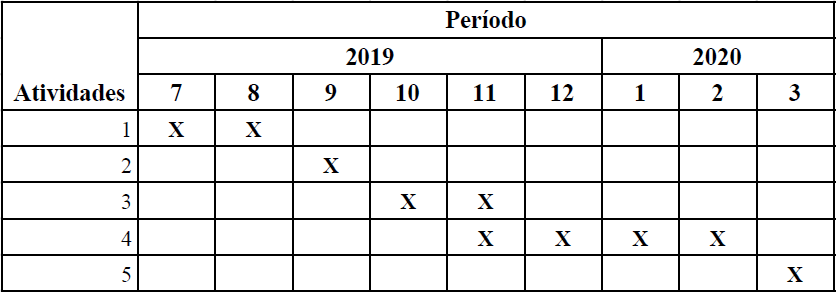
\includegraphics[scale=.7]{figures/crono.PNG}}
%\caption{Gráfico H desenhado pelo participante P14T4}
\label{crono}
\end{figure}
\end{comment}


\begin{table}[!h]
\centering
\def\arraystretch{1.25}
\caption{Cronograma das atividades.}
\label{tab:test3_normality}
\begin{tabular}{|c|c|c|c|c|c|c|c|c|}

\hline

\multirow{ 3}{*}{\textbf{Atividades}}&\multicolumn{8}{c|}{\textbf{Período}}\\\cline{2-9}

& \multicolumn{6}{c|}{\textbf{2019}} &\multicolumn{2}{c|}{\textbf{2020}}\\\cline{2-9}

& 07 & 08 & 09 & 10 & 11 & 12 & 01 & 02\\
\hline

1 & \cellcolor{green!25}$\times$& \cellcolor{green!25}$\times$ & \cellcolor{green!25}$\times$ & \cellcolor{green!25}$\times$ & \cellcolor{green!25}$\times$ & \cellcolor{green!25}$\times$ &\cellcolor{green!25}$\times$ &~\\

%-----------------

2 & \cellcolor{green!25}$\times$ & \cellcolor{green!25}$\times$ &~&~&~&~&~&~\\

%-----------------

3 & ~&~&\cellcolor{green!25}$\times$ &~&~&~&~&~\\

%-----------------

4 &~&~&~&\cellcolor{green!25}$\times$&\cellcolor{green!25}$\times$&~&~&~\\


%-----------------

5 &~&~&~&\cellcolor{green!25}$\times$&\cellcolor{green!25}$\times$&\cellcolor{green!25}$\times$&\cellcolor{green!25}$\times$&~\\

%-----------------

6 &~&~&~&~&~&~&~&\cellcolor{green!25}$\times$\\


\hline
\end{tabular}
\end{table}



Definição das atividades a serem desenvolvidas:
\begin{enumerate}
    \item Revisão da literatura sobre tópicos relacionado ao trabalho;
    \item Desenvolvimento do protótipo de interação por voz;
    \item Realização de testes com usuários;
    \item Escrita de artigos;
    \item Escrita de dissertação;
    \item Defesa de dissertação.
\end{enumerate}

\begin{comment}

% tabela com 25 colunas e 15 linhas, caption de tabela vem acima da mesma.


\begin{enumerate}
    \item Levantamento bibliográfico;
    \item Definição do tema;
    \item Definição dos modelos;
    \item Realização de testes com usuários;
    \item Escrita de artigos;
    \item Desenvolvimento da interação por voz;
    \item Escrita de dissertação;
    \item Defesa de dissertação.
\end{enumerate}

\end{comment}




% ----------------------------------------------------------
% Referências bibliográficas
% ----------------------------------------------------------
\bibliography{abntex2-modelo-references}

%\chapter{Modelo PPGCC}

%Sinta-se convidado a participar do projeto \abnTeX! Acesse o site do projeto em \url{http://www.abntex.net.br/}. Também fique livre para conhecer, estudar, alterar e redistribuir o trabalho do \abnTeX, desde que os arquivos modificados tenham seus nomes alterados e que os créditos sejam dados aos autores originais, nos termos da ``The \LaTeX\ Project Public License''\footnote{\url{http://www.latex-project.org/lppl.txt}}.

% ---
% Capitulo com exemplos de comandos inseridos de arquivo externo 
% ---
%%% abtex2-modelo-include-comandos.tex, v-1.9.7 laurocesar
%% Copyright 2012-2018 by abnTeX2 group at http://www.abntex.net.br/ 
%%
%% This work may be distributed and/or modified under the
%% conditions of the LaTeX Project Public License, either version 1.3
%% of this license or (at your option) any later version.
%% The latest version of this license is in
%%   http://www.latex-project.org/lppl.txt
%% and version 1.3 or later is part of all distributions of LaTeX
%% version 2005/12/01 or later.
%%
%% This work has the LPPL maintenance status `maintained'.
%% 
%% The Current Maintainer of this work is the abnTeX2 team, led
%% by Lauro César Araujo. Further information are available on 
%% http://www.abntex.net.br/
%%
%% This work consists of the files abntex2-modelo-include-comandos.tex
%% and abntex2-modelo-img-marca.pdf
%%

% ---
% Este capítulo, utilizado por diferentes exemplos do abnTeX2, ilustra o uso de
% comandos do abnTeX2 e de LaTeX.
% ---
 
\chapter{Resultados de comandos}\label{cap_exemplos}

Isto é uma sinopse de capítulo. A ABNT não traz nenhuma
normatização a respeito desse tipo de resumo, que é mais comum em romances 
e livros técnicos.

% ---
\section{Codificação dos arquivos: UTF8}
% ---

A codificação de todos os arquivos do \abnTeX\ é \texttt{UTF8}. É necessário que
você utilize a mesma codificação nos documentos que escrever, inclusive nos
arquivos de base bibliográficas |.bib|.

% ---
\section{Citações diretas}
\label{sec-citacao}
% ---

\index{citações!diretas}Utilize o ambiente \texttt{citacao} para incluir
citações diretas com mais de três linhas:

\begin{citacao}
As citações diretas, no texto, com mais de três linhas, devem ser
destacadas com recuo de 4 cm da margem esquerda, com letra menor que a do texto
utilizado e sem as aspas. No caso de documentos datilografados, deve-se
observar apenas o recuo \cite[5.3]{NBR10520:2002}.
\end{citacao}

Use o ambiente assim:

\begin{verbatim}
\begin{citacao}
As citações diretas, no texto, com mais de três linhas [...] deve-se observar
apenas o recuo \cite[5.3]{NBR10520:2002}.
\end{citacao}
\end{verbatim}

O ambiente \texttt{citacao} pode receber como parâmetro opcional um nome de
idioma previamente carregado nas opções da classe (\autoref{sec-hifenizacao}). Nesse
caso, o texto da citação é automaticamente escrito em itálico e a hifenização é
ajustada para o idioma selecionado na opção do ambiente. Por exemplo:

\begin{verbatim}
\begin{citacao}[english]
Text in English language in italic with correct hyphenation.
\end{citacao}
\end{verbatim}

Tem como resultado:

\begin{citacao}[english]
Text in English language in italic with correct hyphenation.
\end{citacao}

\index{citações!simples}Citações simples, com até três linhas, devem ser
incluídas com aspas. Observe que em \LaTeX as aspas iniciais são diferentes das
finais: ``Amor é fogo que arde sem se ver''.

% ---
\section{Notas de rodapé}
% ---

As notas de rodapé são detalhadas pela NBR 14724:2011 na seção 5.2.1\footnote{As
notas devem ser digitadas ou datilografadas dentro das margens, ficando
separadas do texto por um espaço simples de entre as linhas e por filete de 5
cm, a partir da margem esquerda. Devem ser alinhadas, a partir da segunda linha
da mesma nota, abaixo da primeira letra da primeira palavra, de forma a destacar
o expoente, sem espaço entre elas e com fonte menor
\cite{NBR14724:2011}}\footnote{Caso uma série de notas sejam
criadas sequencialmente, o \abnTeX\ instrui o \LaTeX\ para que uma vírgula seja
colocada após cada número do expoente que indica a nota de rodapé no corpo do
texto.}\footnote{Verifique se os números do expoente possuem uma vírgula para
dividi-los no corpo do texto.}. 


% ---
\section{Tabelas}
% ---

\index{tabelas}A \autoref{tab-nivinv} é um exemplo de tabela construída em
\LaTeX.

\begin{table}[htb]
\ABNTEXfontereduzida
\caption[Níveis de investigação]{Níveis de investigação.}
\label{tab-nivinv}
\begin{tabular}{p{2.6cm}|p{6.0cm}|p{2.25cm}|p{3.40cm}}
  %\hline
   \textbf{Nível de Investigação} & \textbf{Insumos}  & \textbf{Sistemas de Investigação}  & \textbf{Produtos}  \\
    \hline
    Meta-nível & Filosofia\index{filosofia} da Ciência  & Epistemologia &
    Paradigma  \\
    \hline
    Nível do objeto & Paradigmas do metanível e evidências do nível inferior &
    Ciência  & Teorias e modelos \\
    \hline
    Nível inferior & Modelos e métodos do nível do objeto e problemas do nível inferior & Prática & Solução de problemas  \\
   % \hline
\end{tabular}
\legend{Fonte: \cite{van86}}
\end{table}

Já a \autoref{tabela-ibge} apresenta uma tabela criada conforme o padrão do
\cite{ibge1993} requerido pelas normas da ABNT para documentos técnicos e
acadêmicos.

\begin{table}[htb]
\IBGEtab{%
  \caption{Um Exemplo de tabela alinhada que pode ser longa
  ou curta, conforme padrão IBGE.}%
  \label{tabela-ibge}
}{%
  \begin{tabular}{ccc}
  \toprule
   Nome & Nascimento & Documento \\
  \midrule \midrule
   Maria da Silva & 11/11/1111 & 111.111.111-11 \\
  \midrule 
   João Souza & 11/11/2111 & 211.111.111-11 \\
  \midrule 
   Laura Vicuña & 05/04/1891 & 3111.111.111-11 \\
  \bottomrule
\end{tabular}%
}{%
  \fonte{Produzido pelos autores.}%
  \nota{Esta é uma nota, que diz que os dados são baseados na
  regressão linear.}%
  \nota[Anotações]{Uma anotação adicional, que pode ser seguida de várias
  outras.}%
  }
\end{table}


% ---
\section{Figuras}
% ---

\index{figuras}Figuras podem ser criadas diretamente em \LaTeX,
como o exemplo da \autoref{fig_circulo}.

\begin{figure}[htb]
    \label{fig_circulo}
	\caption{Aliquam arcu neque, ornarein, ullamcorper quis, commodo eu, libero. Fusce sagittis erat at erat tristiquemollis. Maecenas sapien libero, molestie et, lobortis in, sodales eget, dui. Morbiultrices rutrum lorem. Nam elementum ullamcorper leo. Morbi dui. Aliquamsagittis. Nunc placerat. Pellentesque tristique sodales est. Maecenas imperdietlacinia velit. Cras non urna. Morbi eros pede, suscipit ac, varius vel, egestasnon, eros. Praesent malesuada, diam id pretium elementum, eros sem dictumtortor, vel consectetuer odio sem sed wisi.}
	\begin{center}
	    \setlength{\unitlength}{5cm}
		\begin{picture}(1,1)
		\put(0,0){\line(0,1){1}}
		\put(0,0){\line(1,0){1}}
		\put(0,0){\line(1,1){1}}
		\put(0,0){\line(1,2){.5}}
		\put(0,0){\line(1,3){.3333}}
		\put(0,0){\line(1,4){.25}}
		\put(0,0){\line(1,5){.2}}
		\put(0,0){\line(1,6){.1667}}
		\put(0,0){\line(2,1){1}}
		\put(0,0){\line(2,3){.6667}}
		\put(0,0){\line(2,5){.4}}
		\put(0,0){\line(3,1){1}}
		\put(0,0){\line(3,2){1}}
		\put(0,0){\line(3,4){.75}}
		\put(0,0){\line(3,5){.6}}
		\put(0,0){\line(4,1){1}}
		\put(0,0){\line(4,3){1}}
		\put(0,0){\line(4,5){.8}}
		\put(0,0){\line(5,1){1}}
		\put(0,0){\line(5,2){1}}
		\put(0,0){\line(5,3){1}}
		\put(0,0){\line(5,4){1}}
		\put(0,0){\line(5,6){.8333}}
		\put(0,0){\line(6,1){1}}
		\put(0,0){\line(6,5){1}}
		\end{picture}
	\end{center}
	\legend{Fonte: os autores}
\end{figure}

Ou então figuras podem ser incorporadas de arquivos externos, como é o caso da. Se a figura que for incluída se tratar de um diagrama, um gráfico ou uma ilustração que você mesmo produza, priorize o uso de imagens vetoriais no formato PDF. Com isso, o tamanho do arquivo final do trabalho será menor, e as imagens terão uma apresentação melhor, principalmente quando impressas, uma vez que imagens vetorias são perfeitamente escaláveis para qualquer dimensão. Nesse caso, se for utilizar o Microsoft Excel para produzir gráficos, ou o Microsoft Word para produzir ilustrações, exporte-os como PDF e os incorpore ao documento conforme o exemplo abaixo. No entanto, para manter a coerência no uso de software livre (já que você está usando \LaTeX e \abnTeX), teste a ferramenta \textsf{InkScape}\index{InkScape} (\url{http://inkscape.org/}). Ela é uma excelente opção de código-livre para produzir ilustrações vetoriais, similar ao CorelDraw\index{CorelDraw} ou ao Adobe Illustrator\index{Adobe Illustrator}. De todo modo, caso não seja possível utilizar arquivos de imagens como PDF, utilize qualquer outro formato, como
JPEG, GIF, BMP, etc. Nesse caso, você pode tentar aprimorar as imagens incorporadas com o software livre \textsf{Gimp}\index{Gimp} (\url{http://www.gimp.org/}). Ele é uma alternativa livre ao Adobe Photoshop\index{Adobe Photoshop}.

\begin{figure}[htb]
	\caption{\label{fig_grafico}Gráfico produzido em Excel e salvo como PDF}
	\begin{center}
	    \includegraphics[scale=0.5]{figures/VISUAL-VARIABLES-5-valores.png}
	\end{center}
	\legend{Fonte: \cite{araujo2012}}
\end{figure}

% ---
\subsection{Figuras em \emph{minipages}}
% ---

\emph{Minipages} são usadas para inserir textos ou outros elementos em quadros
com tamanhos e posições controladas. Veja o exemplo da
\autoref{fig_minipage_imagem1} e da \autoref{fig_minipage_grafico2}.

\begin{figure}[htb]
 \label{teste}
 \centering
  \begin{minipage}{0.4\textwidth}
    \centering
    \caption{Imagem 1 da minipage} \label{fig_minipage_imagem1}
    
\includegraphics[scale=0.9]{abntex2-modelo-img-marca.pdf}
    \legend{Fonte: Produzido pelos autores}
  \end{minipage}
  \hfill
  \begin{minipage}{0.4\textwidth}
    \centering
    \caption{Grafico 2 da minipage} \label{fig_minipage_grafico2}
    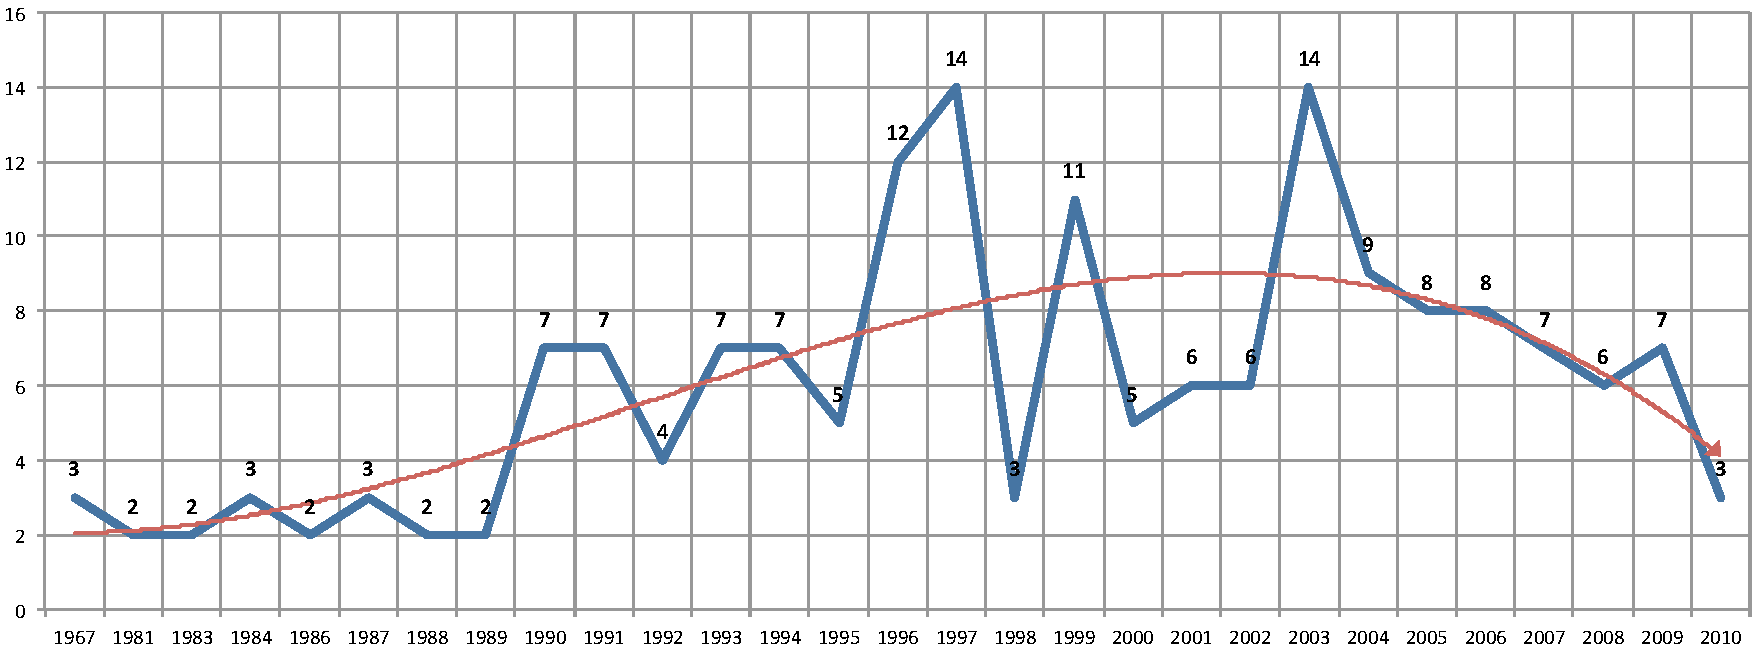
\includegraphics[scale=0.2]{abntex2-modelo-img-grafico.pdf}
    \legend{Fonte: \cite{araujo2012}}
  \end{minipage}
\end{figure}

Observe que, segundo a \cite{NBR14724:2011}, seções 4.2.1.10 e 5.8, as
ilustrações devem sempre ter numeração contínua e única em todo o documento:

\begin{citacao}
Qualquer que seja o tipo de ilustração, sua identificação aparece na parte
superior, precedida da palavra designativa (desenho, esquema, fluxograma,
fotografia, gráfico, mapa, organograma, planta, quadro, retrato, figura,
imagem, entre outros), seguida de seu número de ordem de ocorrência no texto,
em algarismos arábicos, travessão e do respectivo título. Após a ilustração, na
parte inferior, indicar a fonte consultada (elemento obrigatório, mesmo que
seja produção do próprio autor), legenda, notas e outras informações
necessárias à sua compreensão (se houver). A ilustração deve ser citada no
texto e inserida o mais próximo possível do trecho a que se
refere. \cite[seções 5.8]{NBR14724:2011}
\end{citacao}

% ---
\section{Expressões matemáticas}
% ---

\index{expressões matemáticas}Use o ambiente \texttt{equation} para escrever
expressões matemáticas numeradas:

\begin{equation}
  \forall x \in X, \quad \exists \: y \leq \epsilon
\end{equation}

Escreva expressões matemáticas entre \$ e \$, como em $ \lim_{x \to \infty}
\exp(-x) = 0 $, para que fiquem na mesma linha.

Também é possível usar colchetes para indicar o início de uma expressão
matemática que não é numerada.

\[
\left|\sum_{i=1}^n a_ib_i\right|
\le
\left(\sum_{i=1}^n a_i^2\right)^{1/2}
\left(\sum_{i=1}^n b_i^2\right)^{1/2}
\]

Consulte mais informações sobre expressões matemáticas em
\url{https://github.com/abntex/abntex2/wiki/Referencias}.

% ---
\section{Enumerações: alíneas e subalíneas}
% ---

\index{alíneas}\index{subalíneas}\index{incisos}Quando for necessário enumerar
os diversos assuntos de uma seção que não possua título, esta deve ser
subdividida em alíneas \cite[4.2]{NBR6024:2012}:

\begin{alineas}

  \item os diversos assuntos que não possuam título próprio, dentro de uma mesma
  seção, devem ser subdivididos em alíneas; 
  
  \item o texto que antecede as alíneas termina em dois pontos;
  \item as alíneas devem ser indicadas alfabeticamente, em letra minúscula,
  seguida de parêntese. Utilizam-se letras dobradas, quando esgotadas as
  letras do alfabeto;

  \item as letras indicativas das alíneas devem apresentar recuo em relação à
  margem esquerda;

  \item o texto da alínea deve começar por letra minúscula e terminar em
  ponto-e-vírgula, exceto a última alínea que termina em ponto final;

  \item o texto da alínea deve terminar em dois pontos, se houver subalínea;

  \item a segunda e as seguintes linhas do texto da alínea começa sob a
  primeira letra do texto da própria alínea;
  
  \item subalíneas \cite[4.3]{NBR6024:2012} devem ser conforme as alíneas a
  seguir:

  \begin{alineas}
     \item as subalíneas devem começar por travessão seguido de espaço;

     \item as subalíneas devem apresentar recuo em relação à alínea;

     \item o texto da subalínea deve começar por letra minúscula e terminar em
     ponto-e-vírgula. A última subalínea deve terminar em ponto final, se não
     houver alínea subsequente;

     \item a segunda e as seguintes linhas do texto da subalínea começam sob a
     primeira letra do texto da própria subalínea.
  \end{alineas}
  
  \item no \abnTeX\ estão disponíveis os ambientes \texttt{incisos} e
  \texttt{subalineas}, que em suma são o mesmo que se criar outro nível de
  \texttt{alineas}, como nos exemplos à seguir:
  
  \begin{incisos}
    \item \textit{Um novo inciso em itálico};
  \end{incisos}
  
  \item Alínea em \textbf{negrito}:
  
  \begin{subalineas}
    \item \textit{Uma subalínea em itálico};
    \item \underline{\textit{Uma subalínea em itálico e sublinhado}}; 
  \end{subalineas}
  
  \item Última alínea com \emph{ênfase}.
  
\end{alineas}

% ---
\section{Espaçamento entre parágrafos e linhas}
% ---

\index{espaçamento!dos parágrafos}O tamanho do parágrafo, espaço entre a margem
e o início da frase do parágrafo, é definido por:

\begin{verbatim}
   \setlength{\parindent}{1.3cm}
\end{verbatim}

\index{espaçamento!do primeiro parágrafo}Por padrão, não há espaçamento no
primeiro parágrafo de cada início de divisão do documento
(\autoref{sec-divisoes}). Porém, você pode definir que o primeiro parágrafo
também seja indentado, como é o caso deste documento. Para isso, apenas inclua o
pacote \textsf{indentfirst} no preâmbulo do documento:

\begin{verbatim}
   \usepackage{indentfirst}      % Indenta o primeiro parágrafo de cada seção.
\end{verbatim}

\index{espaçamento!entre os parágrafos}O espaçamento entre um parágrafo e outro
pode ser controlado por meio do comando:

\begin{verbatim}
  \setlength{\parskip}{0.2cm}  % tente também \onelineskip
\end{verbatim}

\index{espaçamento!entre as linhas}O controle do espaçamento entre linhas é
definido por:

\begin{verbatim}
  \OnehalfSpacing       % espaçamento um e meio (padrão); 
  \DoubleSpacing        % espaçamento duplo
  \SingleSpacing        % espaçamento simples	
\end{verbatim}

Para isso, também estão disponíveis os ambientes:

\begin{verbatim}
  \begin{SingleSpace} ...\end{SingleSpace}
  \begin{Spacing}{hfactori} ... \end{Spacing}
  \begin{OnehalfSpace} ... \end{OnehalfSpace}
  \begin{OnehalfSpace*} ... \end{OnehalfSpace*}
  \begin{DoubleSpace} ... \end{DoubleSpace}
  \begin{DoubleSpace*} ... \end{DoubleSpace*} 
\end{verbatim}

Para mais informações, consulte \cite{memoir}.

% ---
\section{Inclusão de outros arquivos}\label{sec-include}
% ---

É uma boa prática dividir o seu documento em diversos arquivos, e não
apenas escrever tudo em um único. Esse recurso foi utilizado neste
documento. Para incluir diferentes arquivos em um arquivo principal,
de modo que cada arquivo incluído fique em uma página diferente, utilize o
comando:

\begin{verbatim}
   \include{documento-a-ser-incluido}      % sem a extensão .tex
\end{verbatim}

Para incluir documentos sem quebra de páginas, utilize:

\begin{verbatim}
   \input{documento-a-ser-incluido}      % sem a extensão .tex
\end{verbatim}

% ---
\section{Compilar o documento \LaTeX}
% ---

Geralmente os editores \LaTeX, como o
TeXlipse\footnote{\url{http://texlipse.sourceforge.net/}}, o
Texmaker\footnote{\url{http://www.xm1math.net/texmaker/}}, entre outros,
compilam os documentos automaticamente, de modo que você não precisa se
preocupar com isso.

No entanto, você pode compilar os documentos \LaTeX usando os seguintes
comandos, que devem ser digitados no \emph{Prompt de Comandos} do Windows ou no
\emph{Terminal} do Mac ou do Linux:

\begin{verbatim}
   pdflatex ARQUIVO_PRINCIPAL.tex
   bibtex ARQUIVO_PRINCIPAL.aux
   makeindex ARQUIVO_PRINCIPAL.idx 
   makeindex ARQUIVO_PRINCIPAL.nlo -s nomencl.ist -o ARQUIVO_PRINCIPAL.nls
   pdflatex ARQUIVO_PRINCIPAL.tex
   pdflatex ARQUIVO_PRINCIPAL.tex
\end{verbatim}

% ---
\section{Remissões internas}
% ---

Ao nomear a \autoref{tab-nivinv} e a \autoref{fig_circulo}, apresentamos um
exemplo de remissão interna, que também pode ser feita quando indicamos o
\autoref{cap_exemplos}, que tem o nome \emph{\nameref{cap_exemplos}}. O número
do capítulo indicado é \ref{cap_exemplos}, que se inicia à
\autopageref{cap_exemplos}\footnote{O número da página de uma remissão pode ser
obtida também assim:
\pageref{cap_exemplos}.}.
Veja a \autoref{sec-divisoes} para outros exemplos de remissões internas entre
seções, subseções e subsubseções.

O código usado para produzir o texto desta seção é:

\begin{verbatim}
Ao nomear a \autoref{tab-nivinv} e a \autoref{fig_circulo}, apresentamos um
exemplo de remissão interna, que também pode ser feita quando indicamos o
\autoref{cap_exemplos}, que tem o nome \emph{\nameref{cap_exemplos}}. O número
do capítulo indicado é \ref{cap_exemplos}, que se inicia à
\autopageref{cap_exemplos}\footnote{O número da página de uma remissão pode ser
obtida também assim:
\pageref{cap_exemplos}.}.
Veja a \autoref{sec-divisoes} para outros exemplos de remissões internas entre
seções, subseções e subsubseções.
\end{verbatim}

% ---
\section{Divisões do documento: seção}\label{sec-divisoes}
% ---

Esta seção testa o uso de divisões de documentos. Esta é a
\autoref{sec-divisoes}. Veja a \autoref{sec-divisoes-subsection}.

\subsection{Divisões do documento: subseção}\label{sec-divisoes-subsection}

Isto é uma subseção. Veja a \autoref{sec-divisoes-subsubsection}, que é uma
\texttt{subsubsection} do \LaTeX, mas é impressa chamada de ``subseção'' porque
no Português não temos a palavra ``subsubseção''.

\subsubsection{Divisões do documento: subsubseção}
\label{sec-divisoes-subsubsection}

Isto é uma subsubseção.

\subsubsection{Divisões do documento: subsubseção}

Isto é outra subsubseção.

\subsection{Divisões do documento: subseção}\label{sec-exemplo-subsec}

Isto é uma subseção.

\subsubsection{Divisões do documento: subsubseção}

Isto é mais uma subsubseção da \autoref{sec-exemplo-subsec}.


\subsubsubsection{Esta é uma subseção de quinto
nível}\label{sec-exemplo-subsubsubsection}

Esta é uma seção de quinto nível. Ela é produzida com o seguinte comando:

\begin{verbatim}
\subsubsubsection{Esta é uma subseção de quinto
nível}\label{sec-exemplo-subsubsubsection}
\end{verbatim}

\subsubsubsection{Esta é outra subseção de quinto nível}\label{sec-exemplo-subsubsubsection-outro}

Esta é outra seção de quinto nível.


\paragraph{Este é um parágrafo numerado}\label{sec-exemplo-paragrafo}

Este é um exemplo de parágrafo nomeado. Ele é produzida com o comando de
parágrafo:

\begin{verbatim}
\paragraph{Este é um parágrafo nomeado}\label{sec-exemplo-paragrafo}
\end{verbatim}

A numeração entre parágrafos numeradaos e subsubsubseções são contínuas.

\paragraph{Esta é outro parágrafo numerado}\label{sec-exemplo-paragrafo-outro}

Esta é outro parágrafo nomeado.

% ---
\section{Este é um exemplo de nome de seção longo. Ele deve estar
alinhado à esquerda e a segunda e demais linhas devem iniciar logo abaixo da
primeira palavra da primeira linha}
% ---

Isso atende à norma \cite{NBR14724:2011} seções de 5.2.2 a 5.2.4 
 e \cite{NBR6024:2012} seções de 3.1 a 3.8.

% ---
\section{Diferentes idiomas e hifenizações}
\label{sec-hifenizacao}
% ---

Para usar hifenizações de diferentes idiomas, inclua nas opções do documento o
nome dos idiomas que o seu texto contém. Por exemplo (para melhor
visualização, as opções foram quebras em diferentes linhas):

\begin{verbatim}
\documentclass[
	12pt,
	openright,
	twoside,
	a4paper,
	english,
	french,
	spanish,
	brazil
	]{abntex2}
\end{verbatim}

O idioma português-brasileiro (\texttt{brazil}) é incluído automaticamente pela
classe \textsf{abntex2}. Porém, mesmo assim a opção \texttt{brazil} deve ser
informada como a última opção da classe para que todos os pacotes reconheçam o
idioma. Vale ressaltar que a última opção de idioma é a utilizada por padrão no
documento. Desse modo, caso deseje escrever um texto em inglês que tenha
citações em português e em francês, você deveria usar o preâmbulo como abaixo:

\begin{verbatim}
\documentclass[
	12pt,
	openright,
	twoside,
	a4paper,
	french,
	brazil,
	english
	]{abntex2}
\end{verbatim}

A lista completa de idiomas suportados, bem como outras opções de hifenização,
estão disponíveis em \cite{babel} p. 5-6.

Exemplo de hifenização em inglês\footnote{Extraído de:
\url{http://en.wikibooks.org/wiki/LaTeX/Internationalization}}:

\begin{otherlanguage*}{english}
\textit{Text in English language. This environment switches all language-related
definitions, like the language specific names for figures, tables etc. to the other
language. The starred version of this environment typesets the main text
according to the rules of the other language, but keeps the language specific
string for ancillary things like figures, in the main language of the document.
The environment hyphenrules switches only the hyphenation patterns used; it can
also be used to disallow hyphenation by using the language name
`nohyphenation'.}
\end{otherlanguage*}

Exemplo de hifenização em francês\footnote{Extraído de:
\url{http://bigbrowser.blog.lemonde.fr/2013/02/17/tu-ne-tweeteras-point-le-vatican-interdit-aux-cardinaux-de-tweeter-pendant-le-conclave/}}:

\begin{otherlanguage*}{french}
\textit{Texte en français. Pas question que Twitter ne vienne faire une
concurrence déloyale à la traditionnelle fumée blanche qui marque l'élection
d'un nouveau pape. Pour éviter toute fuite précoce, le Vatican a donc pris un
peu d'avance, et a déjà interdit aux cardinaux qui prendront part au vote
d'utiliser le réseau social, selon Catholic News Service. Une mesure valable
surtout pour les neuf cardinaux – sur les 117 du conclave – pratiquants très
actifs de Twitter, qui auront interdiction pendant toute la période de se
connecter à leur compte.}
\end{otherlanguage*}

Pequeno texto em espanhol\footnote{Extraído de:
\url{http://internacional.elpais.com/internacional/2013/02/17/actualidad/1361102009_913423.html}}:

\foreignlanguage{spanish}{\textit{Decenas de miles de personas ovacionan al pontífice en su
penúltimo ángelus dominical, el primero desde que anunciase su renuncia. El Papa se
centra en la crítica al materialismo}}.

O idioma geral do texto por ser alterado como no exemplo seguinte:

\begin{verbatim}
  \selectlanguage{english}
\end{verbatim}

Isso altera automaticamente a hifenização e todos os nomes constantes de
referências do documento para o idioma inglês. Consulte o manual da classe
\cite{abntex2classe} para obter orientações adicionais sobre internacionalização de
documentos produzidos com \abnTeX.

A \autoref{sec-citacao} descreve o ambiente \texttt{citacao} que pode receber
como parâmetro um idioma a ser usado na citação.

% ---
\section{Consulte o manual da classe \textsf{abntex2}}
% ---

Consulte o manual da classe \textsf{abntex2} \cite{abntex2classe} para uma
referência completa das macros e ambientes disponíveis. 

Além disso, o manual possui informações adicionais sobre as normas ABNT
observadas pelo \abnTeX\ e considerações sobre eventuais requisitos específicos
não atendidos, como o caso da \cite{NBR14724:2011} seção 5.2.2, que
especifica o espaçamento entre os capítulos e o início do texto, regra
propositalmente não atendida pelo presente modelo.

% ---
\section{Referências bibliográficas}
% ---

A formatação das referências bibliográficas conforme as regras da ABNT são um
dos principais objetivos do \abnTeX. Consulte os manuais
\cite{abntex2cite} e \cite{abntex2cite-alf} para obter informações
sobre como utilizar as referências bibliográficas.

%-
\subsection{Acentuação de referências bibliográficas}
%-

Normalmente não há problemas em usar caracteres acentuados em arquivos
bibliográficos (\texttt{*.bib}). Porém, como as regras da ABNT fazem uso quase
abusivo da conversão para letras maiúsculas, é preciso observar o modo como se
escreve os nomes dos autores. Na ~\autoref{tabela-acentos} você encontra alguns
exemplos das conversões mais importantes. Preste atenção especial para `ç' e `í'
que devem estar envoltos em chaves. A regra geral é sempre usar a acentuação
neste modo quando houver conversão para letras maiúsculas.

\begin{table}[htbp]
\caption{Tabela de conversão de acentuação.}
\label{tabela-acentos}

\begin{center}
\begin{tabular}{ll}\hline\hline
acento & \textsf{bibtex}\\
à á ã & \verb+\`a+ \verb+\'a+ \verb+\~a+\\
í & \verb+{\'\i}+\\
ç & \verb+{\c c}+\\
\hline\hline
\end{tabular}
\end{center}
\end{table}


% ---
\section{Precisa de ajuda?}
% ---

Consulte a FAQ com perguntas frequentes e comuns no portal do \abnTeX:
\url{https://github.com/abntex/abntex2/wiki/FAQ}.

Inscreva-se no grupo de usuários \LaTeX:
\url{http://groups.google.com/group/latex-br}, tire suas dúvidas e ajude
outros usuários.

Participe também do grupo de desenvolvedores do \abnTeX:
\url{http://groups.google.com/group/abntex2} e faça sua contribuição à
ferramenta.

% ---
\section{Você pode ajudar?}
% ---

Sua contribuição é muito importante! Você pode ajudar na divulgação, no
desenvolvimento e de várias outras formas. Veja como contribuir com o \abnTeX\
em \url{https://github.com/abntex/abntex2/wiki/Como-Contribuir}.

% ---
\section{Quer customizar os modelos do \abnTeX\ para sua instituição ou
universidade?}
% ---

Veja como customizar o \abnTeX\ em:
\url{https://github.com/abntex/abntex2/wiki/ComoCustomizar}.


% ---

% ----------------------------------------------------------
% Finaliza a parte no bookmark do PDF
% para que se inicie o bookmark na raiz
% e adiciona espaço de parte no Sumário
% ----------------------------------------------------------
\phantompart

% ----------------------------------------------------------
% ELEMENTOS PÓS-TEXTUAIS
% ----------------------------------------------------------
\postextual
% ----------------------------------------------------------

% ----------------------------------------------------------
% Glossário
% ----------------------------------------------------------
%
% Consulte o manual da classe abntex2 para orientações sobre o glossário.
%
%\glossary

% ----------------------------------------------------------
%Apêndices
% ----------------------------------------------------------

% ---
% Inicia os apêndices
% ---

% ---

\end{document}
